\documentclass[a4paper,12pt]{report}

% Codifica, lingua, font
\usepackage[utf8]{inputenc}
\usepackage[T1]{fontenc}
\usepackage[italian]{babel}
\usepackage{lmodern}

% Impaginazione
\usepackage{geometry}

% Grafica, colori, tabelle, float
\usepackage{graphicx}
\usepackage{float}
\usepackage[table]{xcolor}
\usepackage{tabularx}

% Matematica
\usepackage{amsmath}

% Verbatim e listing
\usepackage{fancyvrb}
\usepackage{alltt}
\usepackage{listings}

% Liste
% \usepackage{enumitem}

% Link e riferimenti intelligenti (hyperref prima di cleveref)
\usepackage{hyperref}
% \usepackage[italian]{cleveref}

\geometry{margin=1in}

% colori
\definecolor{codegray}{rgb}{0.5,0.5,0.5}
\definecolor{codeBlue}{HTML}{6495ED}
\definecolor{codegreen}{HTML}{12911F}
\definecolor{backcolour}{rgb}{0.95,0.95,0.92}

% stile listings
\lstdefinestyle{sqlstyle}{
    language=SQL,
    backgroundcolor=\color{backcolour},
    commentstyle=\color{codegreen}\itshape,
    keywordstyle=\color{codeBlue}\bfseries,
    numberstyle=\tiny\color{codegray},
    stringstyle=\color{codeBlue},
    basicstyle=\footnotesize\ttfamily,
    breakatwhitespace=false,
    breaklines=true,
    captionpos=b,
    keepspaces=true,
    numbers=left,
    numbersep=10pt,
    showspaces=false,
    showstringspaces=false,
    showtabs=false
}

% ambiente dedicato
\lstnewenvironment{sqlcode}[1][]{
    \lstset{style=sqlstyle,#1}
}{}

\hypersetup{
    colorlinks=false,
    pdfborder={1 1 1},
    linkbordercolor={1 0 0},
    urlbordercolor={1 0 0},
    citebordercolor={1 0 0},
    pdftitle={Elaborato Basi di Dati},
    pdfauthor={Maisam Noumi, Alessandro Rebosio, Filippo Ricciotti}
}

\title{
    \vspace*{2cm}
    \LARGE Relazione per il corso di \\[0.5cm]
    \textit{Basi di Dati} \\[2cm]
    \Huge\textbf{Agriturismo} \\[2cm]
}

\author{
    \Large
    Alessandro Rebosio \\
    Filippo Ricciotti
}

\date{
    \vspace{1cm}
    \today \\[0.5cm]
    Anno Accademico 2024-2025
}

\begin{document}

\maketitle

\tableofcontents

\chapter{Analisi dei requisiti}
\section{Intervista}

L'agriturismo intende dotarsi di una piattaforma digitale che razionalizzi le attività quotidiane 
e migliori l'esperienza dei clienti, integrando in un unico ambiente la gestione del personale, 
la vendita di prodotti e la promozione di eventi. Il titolare desidera uno strumento accessibile 
via web, utilizzabile da utenti registrati e dal personale autorizzato, in grado di offrire una 
visione chiara e centralizzata delle informazioni operative, riducendo errori e tempi di 
coordinamento.

Il cuore dell'applicativo è costituito da un catalogo di prodotti e da un calendario di
eventi, visibili ai visitatori e consultabili dagli utenti registrati. I prodotti, identificati 
da un codice univoco, sono descritti da un nome e da un prezzo, con la garanzia che i valori 
economici rimangano sempre positivi. Gli eventi, invece, sono presentati con titolo, 
descrizione, data di svolgimento e un numero di posti disponibili; la loro pubblicazione è 
effettuata da dipendenti autorizzati, così da mantenere controllo e coerenza dell'offerta.

Gli utenti potranno creare un account fornendo un nome utente, un indirizzo email e una 
password; ogni profilo sarà associato a una persona identificata tramite codice fiscale, 
così da assicurare un'anagrafica pulita e non ridondante. Una volta autenticati, gli utenti 
potranno consultare il catalogo, comporre ordini di acquisto di prodotti e completarne la 
registrazione: ogni ordine sarà tracciato con data e ora, e conterrà le righe di dettaglio con 
quantità e prezzo unitario, in modo da consentire il calcolo del totale e la successiva 
rendicontazione. Gli acquisti rimarranno associati in modo permanente all'account dell'utente, 
così da poterli rivedere e analizzare nel tempo.

Per la dimensione esperienziale dell'agriturismo, la piattaforma offrirà una sezione dedicata 
agli eventi: gli utenti interessati potranno iscriversi indicando il numero di partecipanti; il 
sistema dovrà garantire che le prenotazioni non superino i posti disponibili e registrerà 
automaticamente data e ora di ciascuna iscrizione. In questo modo, il titolare potrà monitorare 
in tempo reale l'andamento delle adesioni e prevedere l'affluenza, ottimizzando l'organizzazione 
delle serate e delle attività tematiche.

La gestione del personale rappresenta un altro pilastro del sistema. Ciascun dipendente sarà un 
utente abilitato a funzioni specifiche e caratterizzato da un ruolo (ad esempio sala, cucina, 
reception), con la possibilità di tracciarne lo storico delle variazioni nel tempo. La 
pianificazione dei turni avverrà attraverso la definizione di modelli di turno (per giorno della 
settimana, con orari di inizio e fine) e la loro assegnazione a calendario per una data 
specifica. Ogni assegnazione prevede uno stato — programmato, completato o assente — così da 
fotografare l'effettiva presenza; inoltre, il sistema eviterà conflitti, impedendo che uno 
stesso dipendente risulti assegnato a più turni nella medesima giornata.

Dal punto di vista direzionale, il titolare richiede una reportistica essenziale ma 
affidabile: l'andamento delle vendite per periodo, la partecipazione agli eventi e un quadro 
della presenza/assenza del personale sui turni. La piattaforma dovrà salvaguardare la sicurezza 
dei dati, conservando le password in forma sicura e applicando vincoli di integrità su prezzi e 
quantità; le operazioni frequenti — come consultare il catalogo, registrare un ordine o 
iscriversi a un evento — dovranno risultare rapide e semplici, privilegiando chiarezza e 
immediatezza d'uso.

\section{Estrazione dei concetti principali}

L'agriturismo intende realizzare una piattaforma digitale che unisca in un unico ecosistema la 
vendita di prodotti, la promozione e gestione degli eventi e l'organizzazione del personale. Il 
sistema sarà accessibile via web agli utenti registrati e al personale autorizzato, con 
l'obiettivo di offrire una vista centralizzata e coerente delle attività quotidiane, riducendo 
errori operativi e tempi di coordinamento. Il cuore dell'applicazione è rappresentato da un 
\textbf{catalogo di \underline{prodotti}} e da un calendario \underline{eventi}: i 
\underline{prodotti}, identificati in modo univoco (\textbf{codice}), e descritti da 
\textbf{nome} e \textbf{prezzo}, saranno acquistabili dagli \underline{utenti} autenticati; gli 
\underline{eventi}, caratterizzati da \textbf{titolo}, \textbf{descrizione}, \textbf{data} e 
\textbf{posti disponibili}, saranno visibili e prenotabili secondo regole di capienza stabilite 
dall'azienda.

Gli \underline{utenti} potranno creare un account fornendo \textbf{nome utente}, \textbf{email} 
e \textbf{password}; ogni account sarà associato a una \underline{persona} identificata da 
\textbf{codice fiscale}, in modo da mantenere un'anagrafica solida e priva di duplicati. Una 
volta autenticati, gli \underline{utenti} potranno consultare il catalogo e comporre 
\underline{ordini}, che verranno registrati con \textbf{data} e \textbf{ora} e articolati in 
\underline{righe d'ordine} di dettaglio con \textbf{quantità} e \textbf{prezzo unitario}, 
garantendo la correttezza dei totali e la tracciabilità nel tempo. Gli \underline{acquisti} 
resteranno permanentemente associati al profilo dell'\underline{utente}, consentendo 
storicizzazione e successive analisi gestionali.

La dimensione esperienziale sarà supportata da un modulo \underline{eventi}: la creazione degli 
\underline{eventi} è affidata a \underline{dipendenti} autorizzati e prevede l'indicazione dei 
\textbf{posti disponibili}. Gli \underline{utenti} potranno iscriversi (\underline{iscrizione 
evento}) specificando il \textbf{numero di partecipanti}, mentre il sistema dovrà prevenire 
il superamento della capienza e registrare automaticamente \textbf{data} e \textbf{ora} di ogni 
iscrizione. In parallelo, la gestione interna del \underline{personale} è fondata su 
\underline{ruoli} e \underline{turni}: ogni \underline{dipendente} possiede un \textbf{ruolo} 
corrente, con storico delle variazioni per fini di audit, e partecipa a una pianificazione che 
combina \underline{modelli di turno} (\textbf{giorno della settimana}, \textbf{nome}, 
\textbf{orari}) con \underline{assegnazioni di turno} a calendario per \textbf{date} specifiche. 
Ogni assegnazione registra lo \textbf{stato} effettivo (\textbf{programmato}, 
\textbf{completato}, \textbf{assente}) e impedisce conflitti, evitando che un 
\underline{dipendente} risulti pianificato su più turni nello stesso giorno.

A livello trasversale, la piattaforma tutela integrità e sicurezza dei dati: \textbf{prezzi} e 
\textbf{quantità} devono essere sempre positivi, le relazioni fra \underline{utenti}, 
\underline{dipendenti}, \underline{ordini} ed \underline{eventi} rispettano vincoli 
referenziali, e le informazioni sensibili come le \textbf{password} sono gestite in modo sicuro. 

Il \underline{titolare} dispone di una visione complessiva tramite report essenziali su 
\underline{vendite}, \underline{adesioni agli eventi} e \underline{presenza del personale}, 
mentre l'interfaccia privilegia semplicità e rapidità nelle operazioni più frequenti.

\chapter{Progettazione concettuale}
In questo capitolo presenteremo lo schema ER, partendo da una versione iniziale e migliorandola 
passo dopo passo ad arrivare a quella definitiva, attraverso dei raffinamenti.

\section{Schema iniziale}
Dopo aver eseguito l'analisi del dominio iniziale, abbiamo creato uno schema di base con
le entità e le relazioni principali, che sarà poi perfezionato nei passaggi successivi.
\begin{figure}[H]
	\centering
	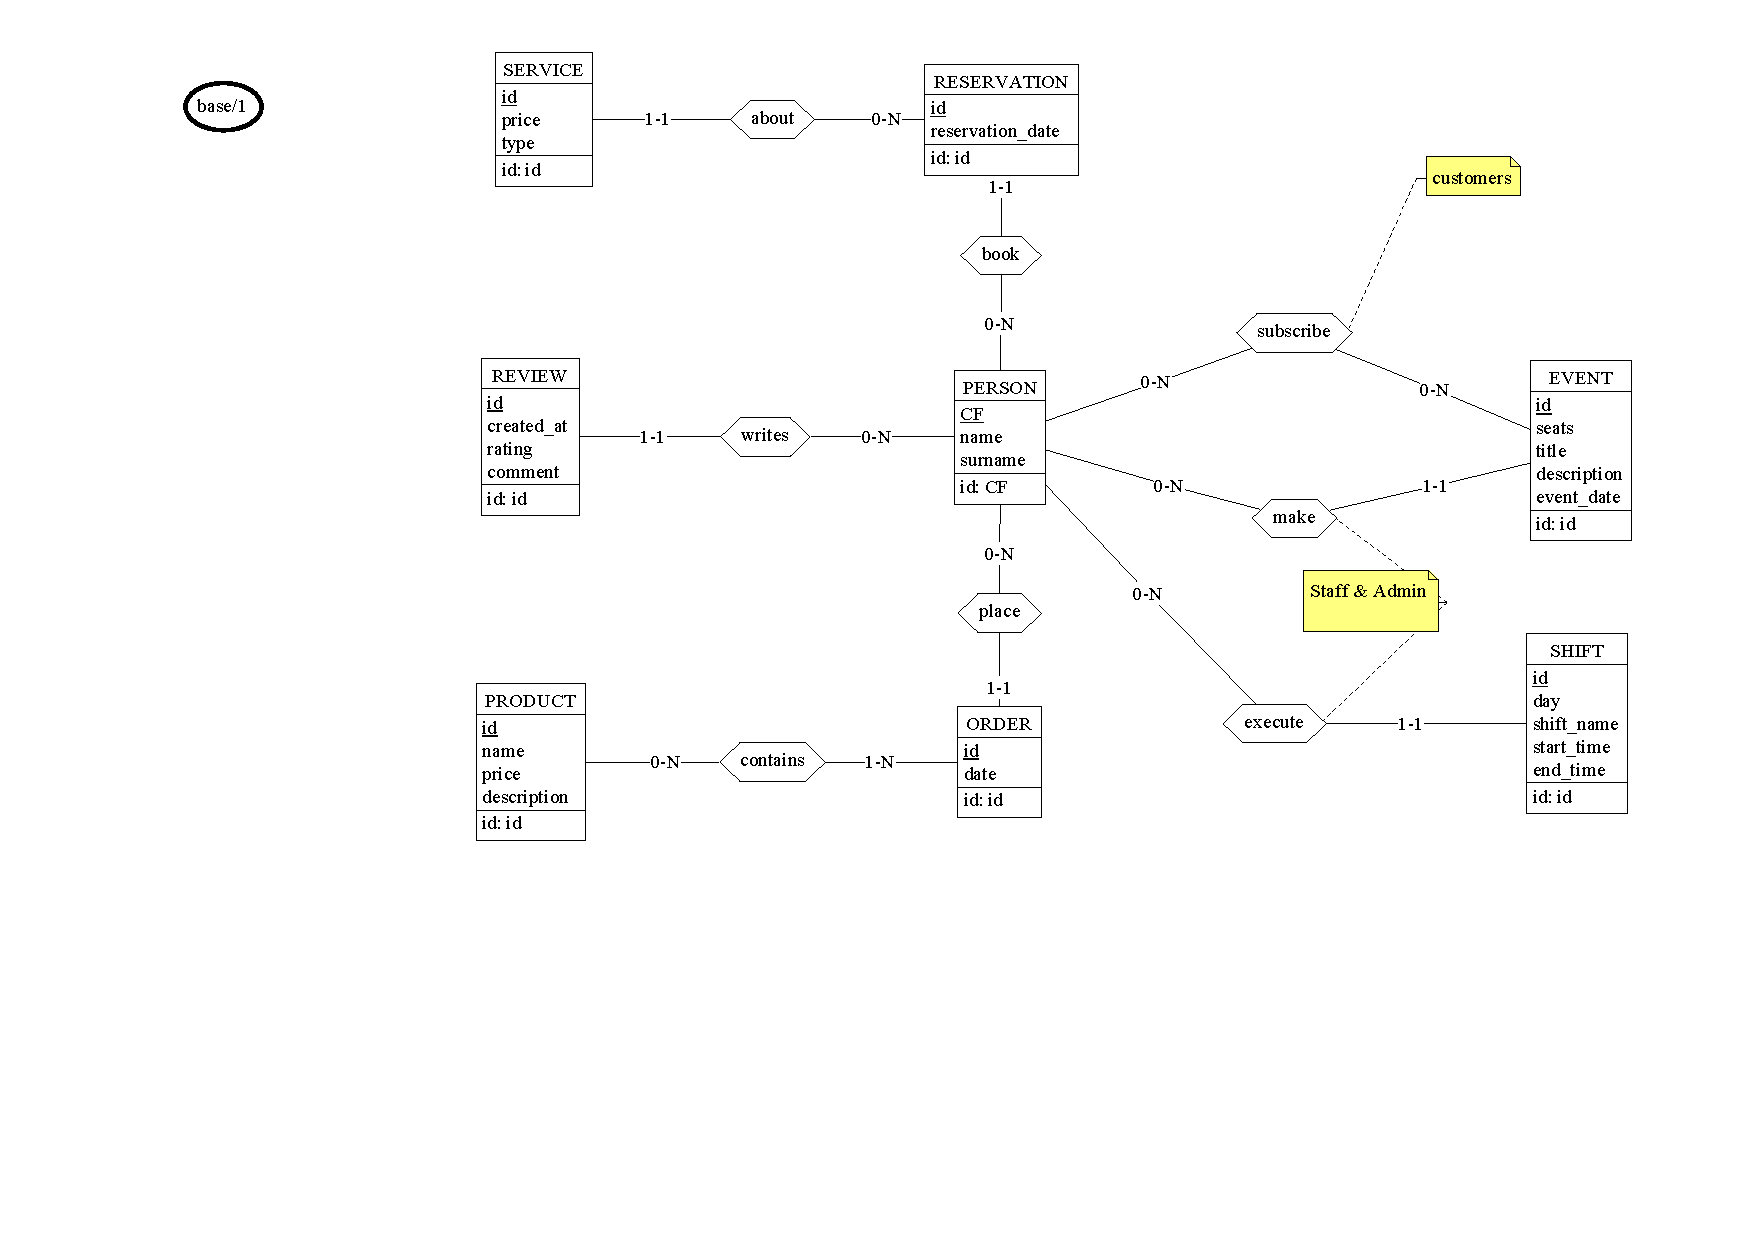
\includegraphics[width=\textwidth, trim=200pt 170pt 50pt 0pt, clip]{./schemas/base.pdf}
	\caption{Schema ER iniziale}
	\label{fig:schema-iniziale}
\end{figure}

\section{Raffinamenti proposti}
\subsection{Utente e Dipendente}
Nel modello concettuale iniziale la \textbf{Persona} raggruppava tutte le possibili interazioni 
con il sistema: iscrizione, creazione di eventi, prenotazioni, ordini e recensioni. Questo 
approccio, sebbene corretto dal punto di vista logico, risultava poco chiaro perché attribuiva 
a un'unica entità responsabilità molto eterogenee.

\vspace{\baselineskip}
Per migliorare la rappresentazione è stato introdotto un raffinamento mediante 
generalizzazione/specializzazione: la superclasse \textbf{Persona} è stata mantenuta per 
raccogliere gli attributi comuni (CF, nome, cognome), mentre le funzionalità specifiche sono 
state assegnate ai sottotipi \textbf{Cliente} e \textbf{Dipendente}.

\vspace{\baselineskip}
In questo modo i clienti gestiscono attività come acquisti, recensioni, ordini e iscrizioni agli 
eventi, mentre i dipendenti si occupano della creazione degli eventi e della gestione dei 
servizi. Tale raffinamento migliora la chiarezza semantica del modello, riduce le ambiguità e 
riflette meglio la separazione dei ruoli reali all'interno del dominio applicativo.

\vspace{\baselineskip}
Il raffinamento mette in evidenza anche le dipendenze temporali (come la gestione dei turni \textbf{Shift} o la cronologia del personale \textbf{Employee History}) e garantisce che ogni operazione rispetti vincoli di consistenza e cardinalità, rendendo il modello complessivo coerente, sicuro e facilmente estendibile.

\begin{figure}[H]
	\centering
	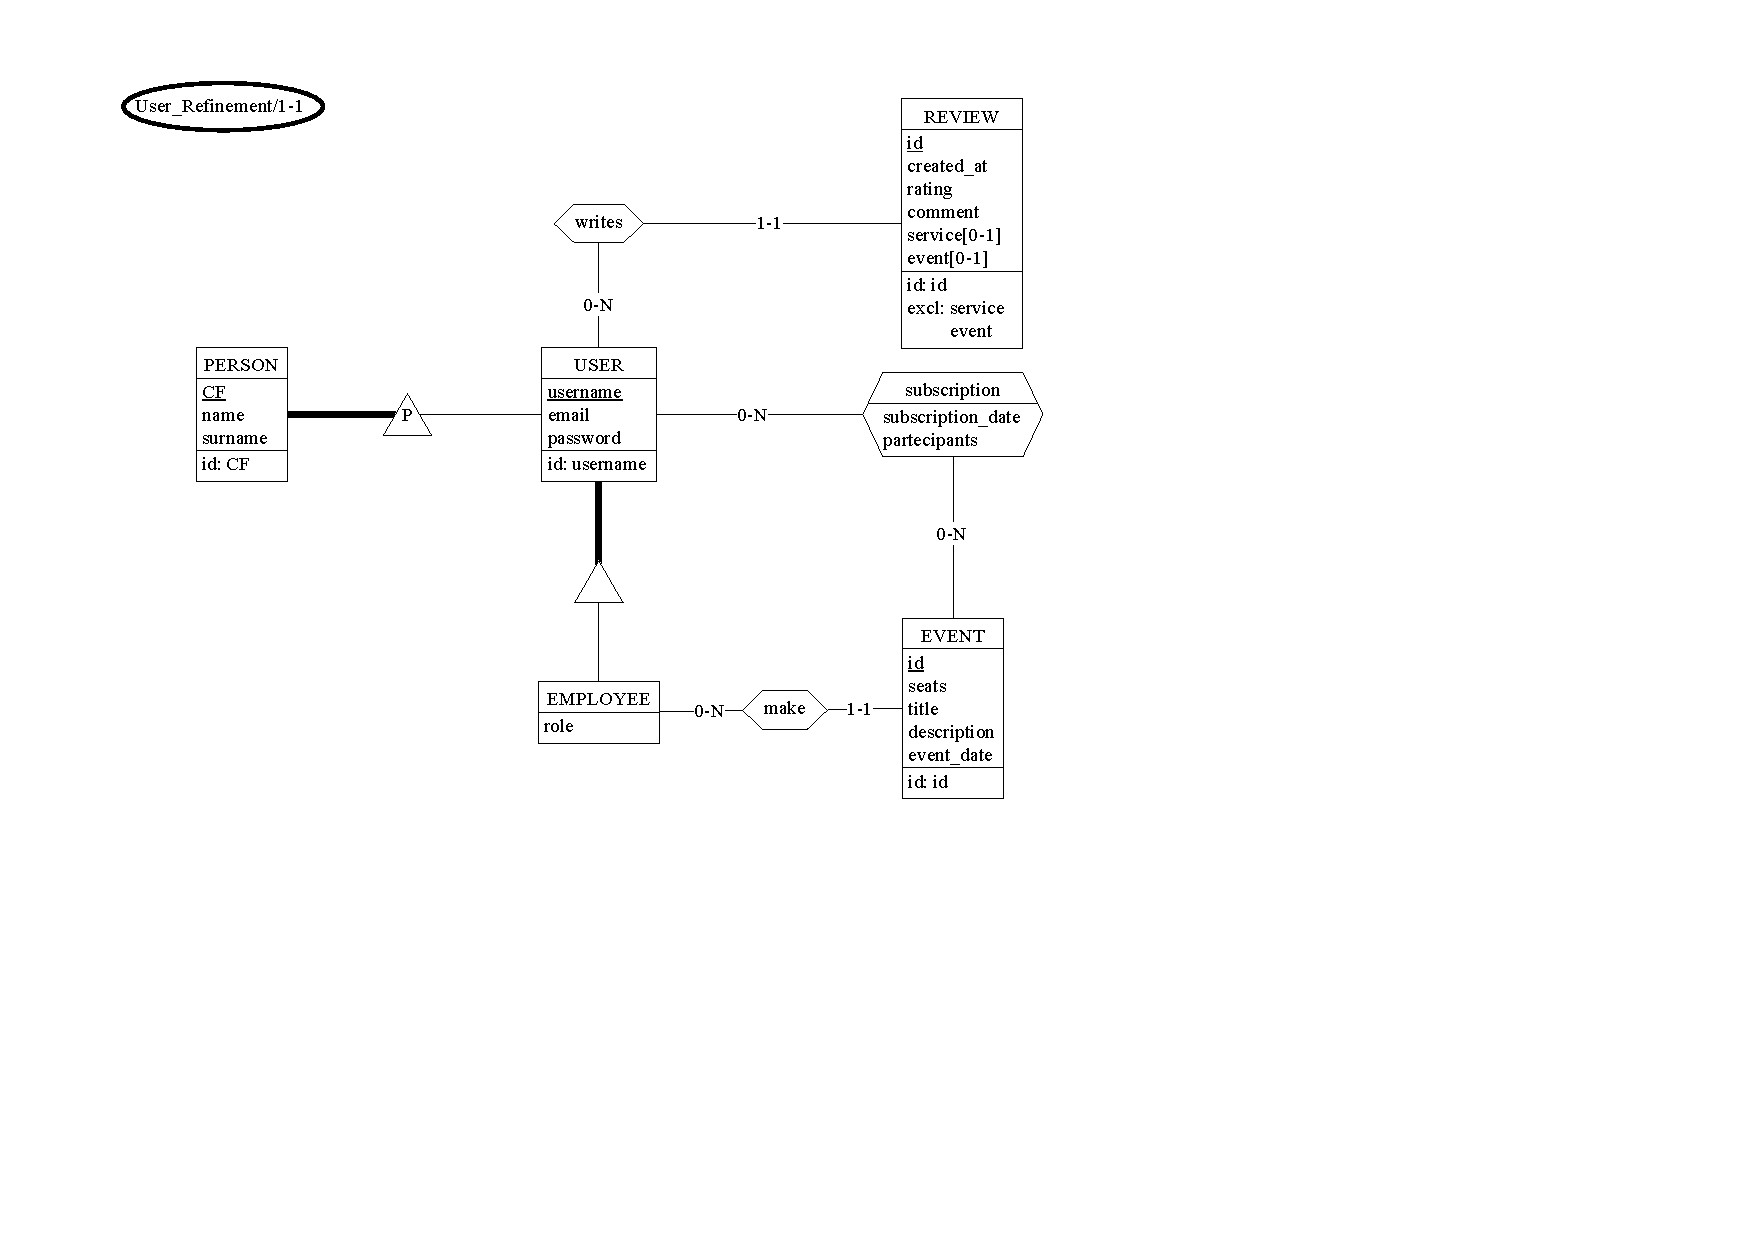
\includegraphics[width=\textwidth, trim=0 200pt 275pt 0, clip]{./schemas/refinements/user.pdf}
	\caption{Raffinamento utente e dipendente}
	\label{fig:raffinamento-utente}
\end{figure}

\newpage
\subsection{Prenotazione Servizi}
Nel modello iniziale i diversi tipi di servizi potevano essere rappresentati come entità 
distinte, con il rischio però di ridondanza e frammentazione dei dati.

\vspace{\baselineskip}
Con il raffinamento si è introdotta una \textbf{generalizzazione}: è stata creata la superclasse 
\textbf{Servizio}, che raccoglie gli attributi comuni (id, price, type), mentre ciascuna 
tipologia specifica di servizio (Camera e Ristorante) è modellata come sottoclasse.

\vspace{\baselineskip}
Inoltre, è stato introdotto il legame con l'entità \textbf{Prenotazione}, che consente di 
registrare le informazioni su data di inizio e fine e di associare ogni prenotazione a uno o 
più servizi specifici tramite la relazione con \textbf{Dettagli Prenotazione}. Questo
raffinamento permette di gestire correttamente scenari in cui un utente prenota più servizi 
differenti nello stesso arco temporale.
\begin{figure}[H]
	\centering
	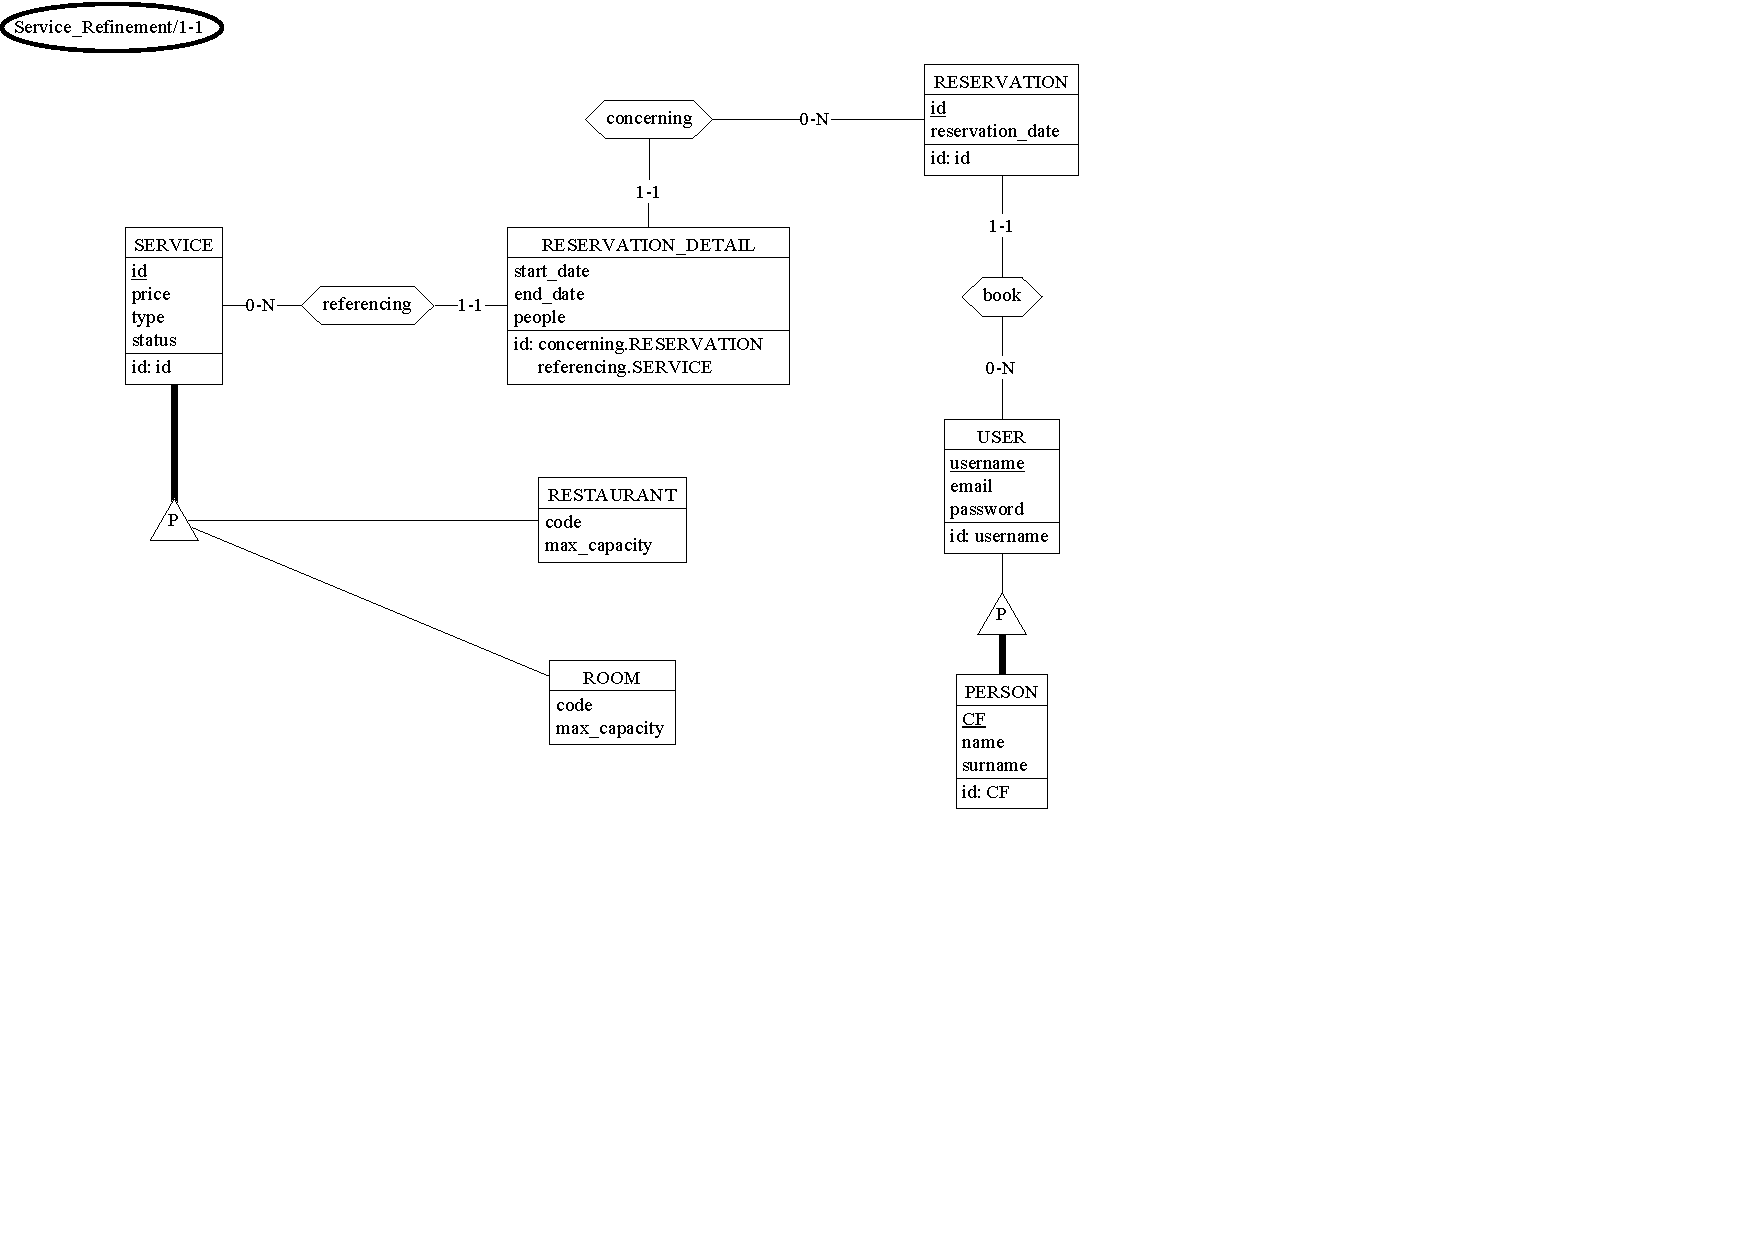
\includegraphics[width=\textwidth, trim=0 200pt 300pt 0, clip]{./schemas/refinements/service.pdf}
	\caption{Raffinamento prenotazione e servizi}
	\label{fig:raffinamento-servizi-prenotazione}
\end{figure}

\newpage
\subsection{Prodotti e ordini}
Nel modello concettuale iniziale, la gestione degli ordini e dei prodotti risultava poco 
dettagliata: un ordine era semplicemente collegato a uno o più prodotti, senza possibilità di 
specificare informazioni aggiuntive come quantità o prezzo unitario.

\vspace{\baselineskip}
Con il raffinamento, è stata introdotta l'entità \textbf{Dettaglio Ordine}, che funge da 
associazione tra \textbf{Ordine} e \textbf{Prodotto}. Ogni dettaglio ordine consente di 
memorizzare, per ciascun prodotto incluso in un ordine, la quantità acquistata e il prezzo 
applicato. Questo permette di rappresentare in modo accurato scenari reali come ordini
multiprodotto, applicazione di sconti o variazioni di prezzo nel tempo.

\vspace{\baselineskip}
Inoltre, viene mantenuta la generalizzazione tra \textbf{Persona} e \textbf{Utente}, già 
introdotta nei raffinamenti precedenti, per distinguere i dati anagrafici comuni da quelli 
specifici per l'accesso al sistema e la gestione degli ordini. Questo approccio migliora la 
flessibilità e la chiarezza del modello, consentendo una gestione più efficace
delle informazioni relative agli acquisti.
\begin{figure}[H]
	\centering
	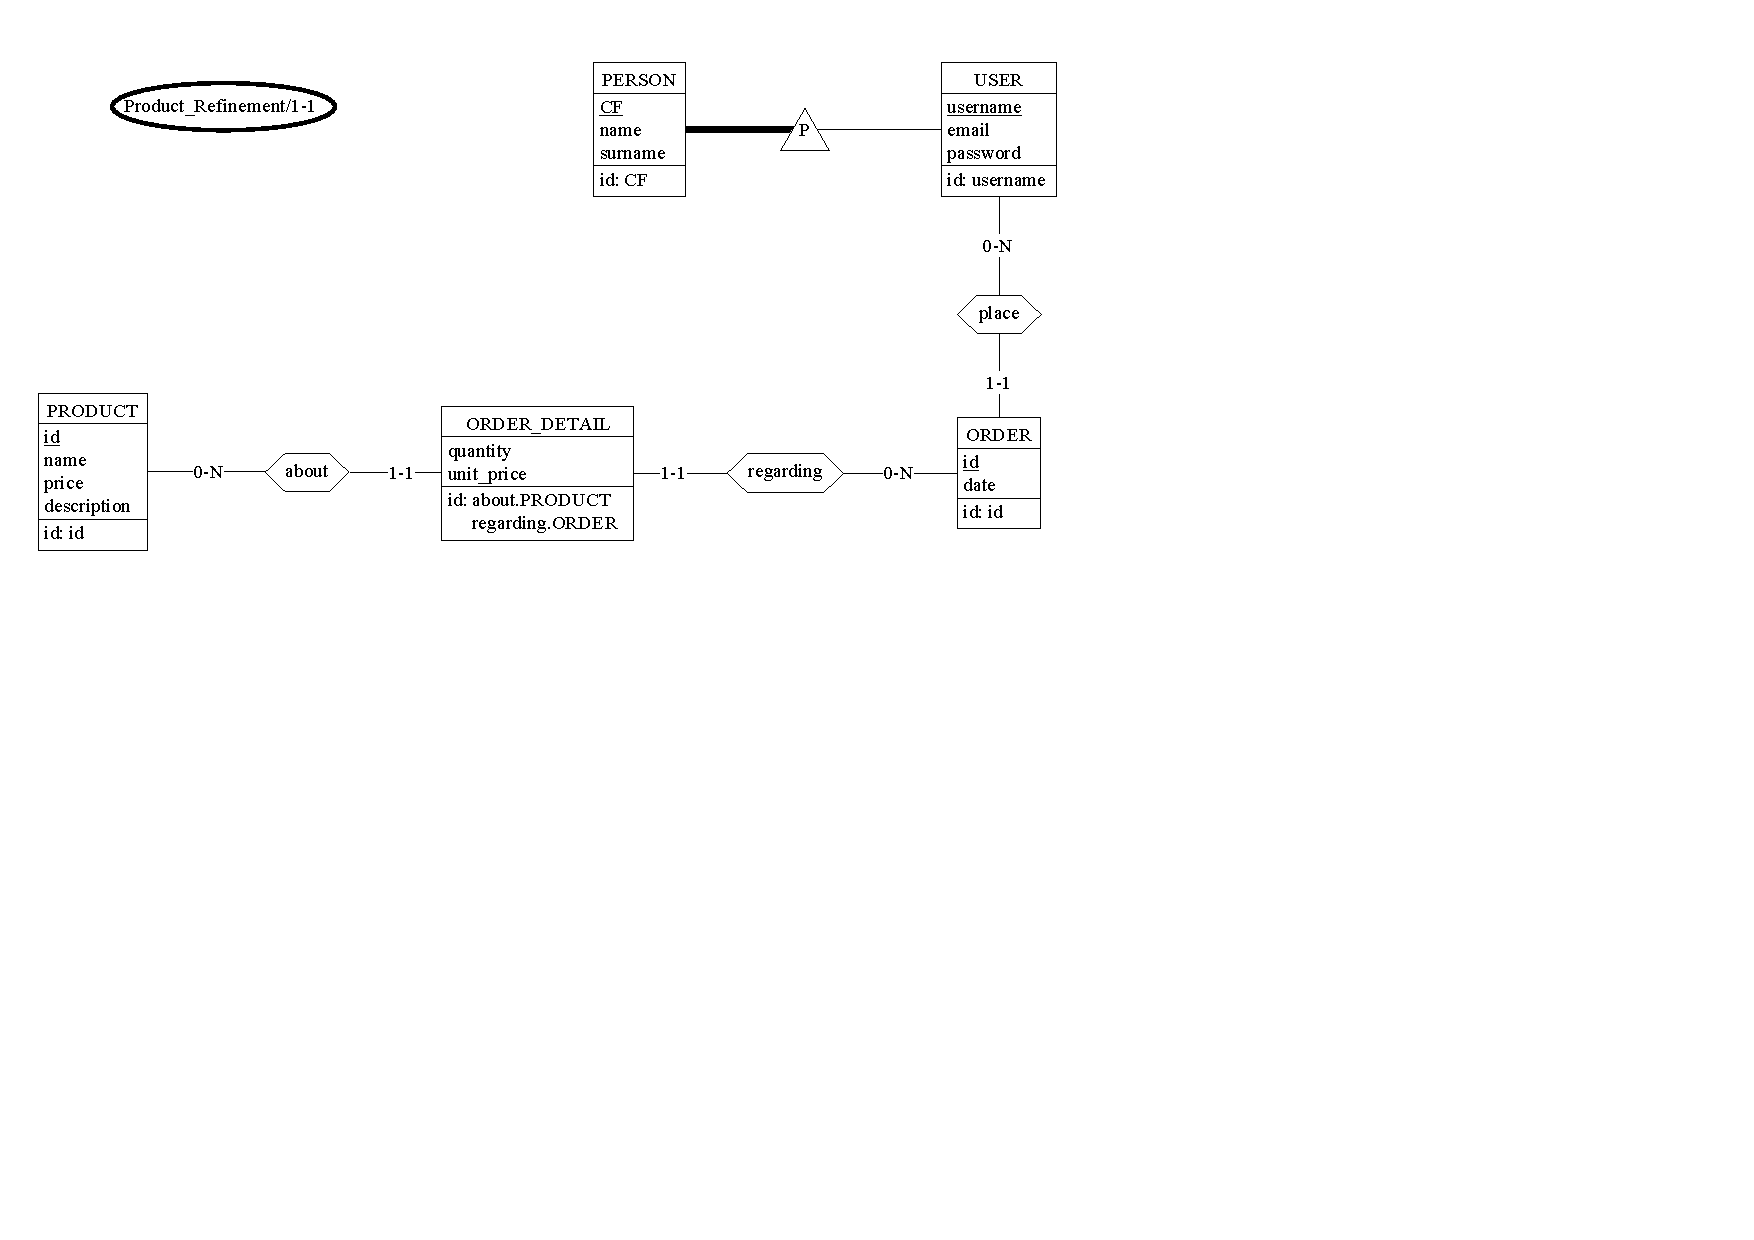
\includegraphics[width=\textwidth, trim=0 300pt 325pt 0, clip]{./schemas/refinements/product.pdf}
	\caption{Raffinamento prodotti e ordini}
	\label{fig:raffinamento-prodotto-ordini}
\end{figure}

\newpage
\section{Schema concettuale finale}
Qui di seguito, è presente lo schema concettuale finale con tutti i raffinamenti.

\begin{figure}[H]
    \centering
    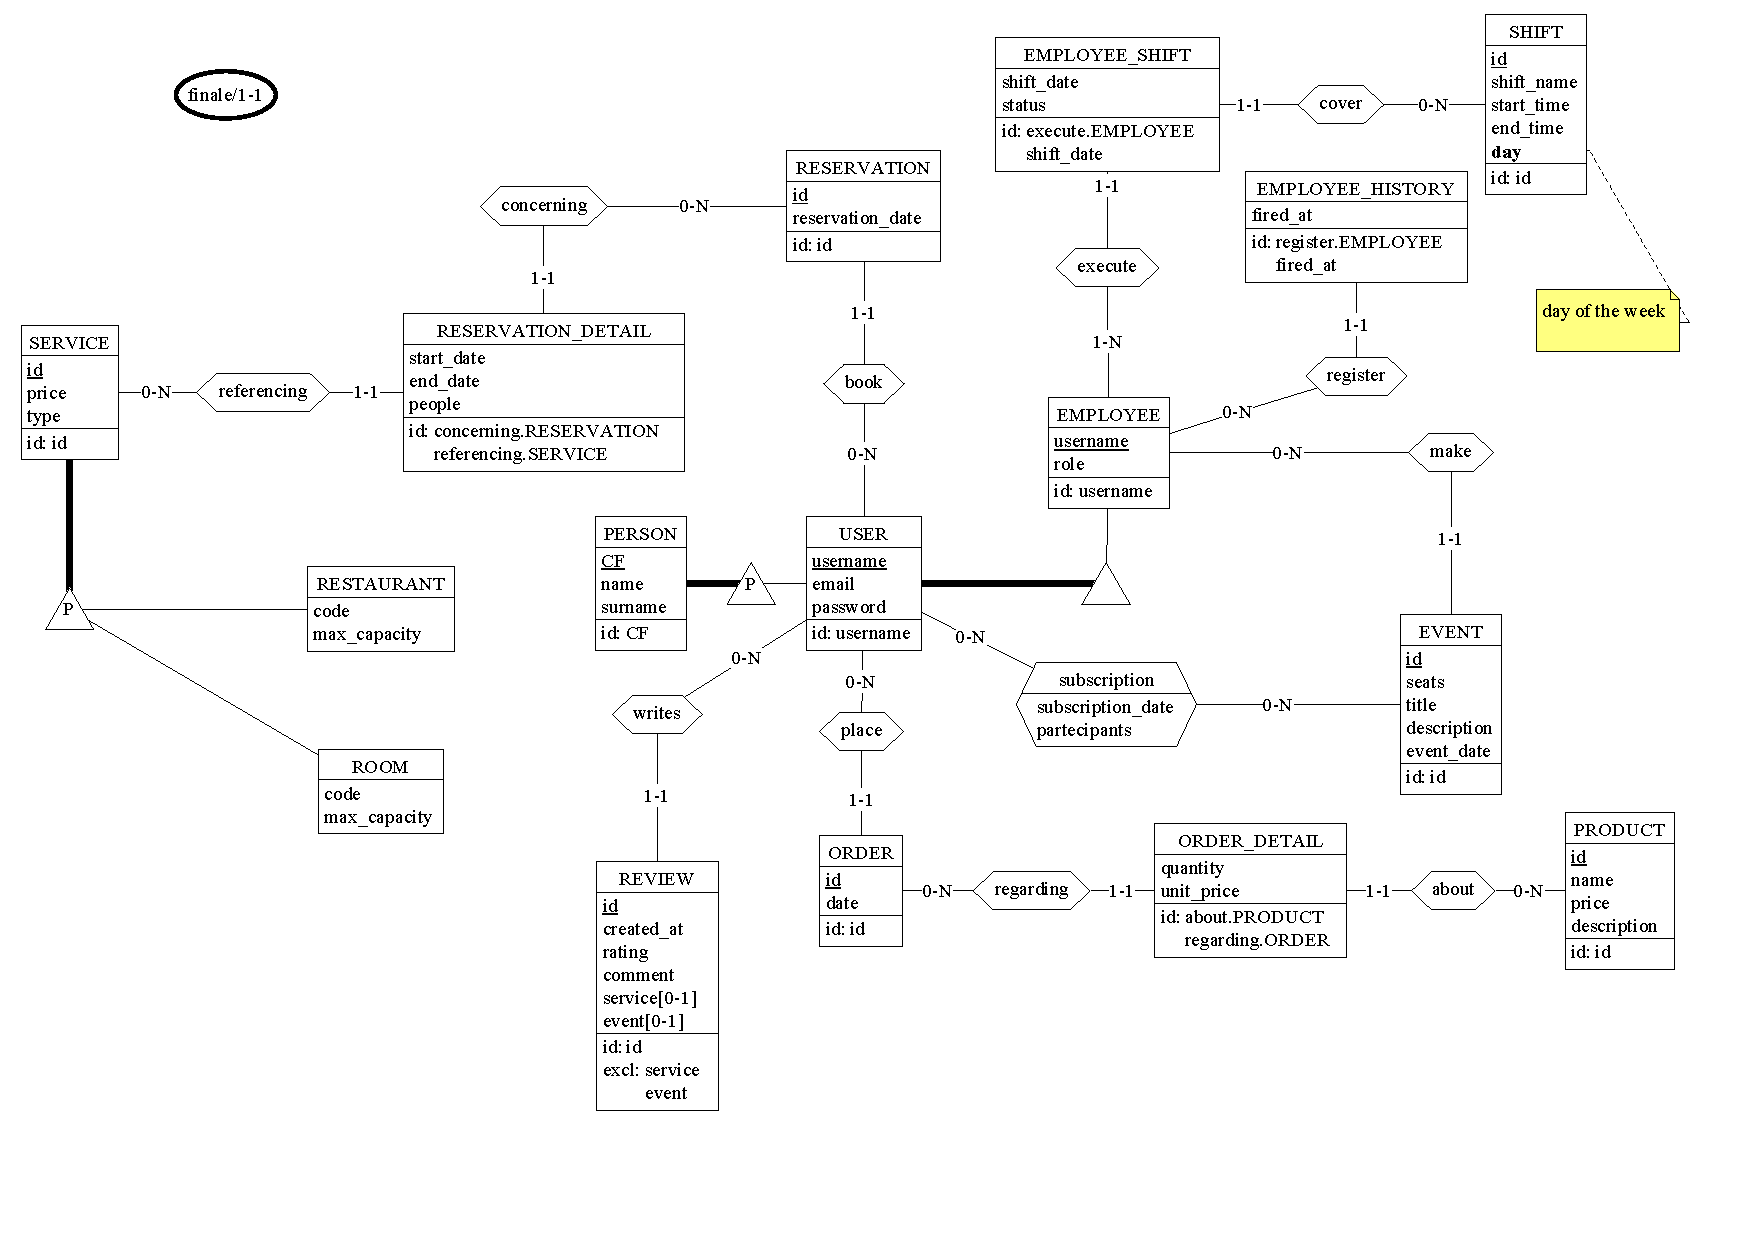
\includegraphics[width=\textwidth, trim=0 0 0 0]{./schemas/refinements/final.pdf}
    \caption{Schema ER, schema concettuale finale}
    \label{fig:schema-finale}
\end{figure}
\newpage

\chapter{Progettazione Logica}

\section{Schema relazionale finale}
\begin{figure}[H]
    \centering
    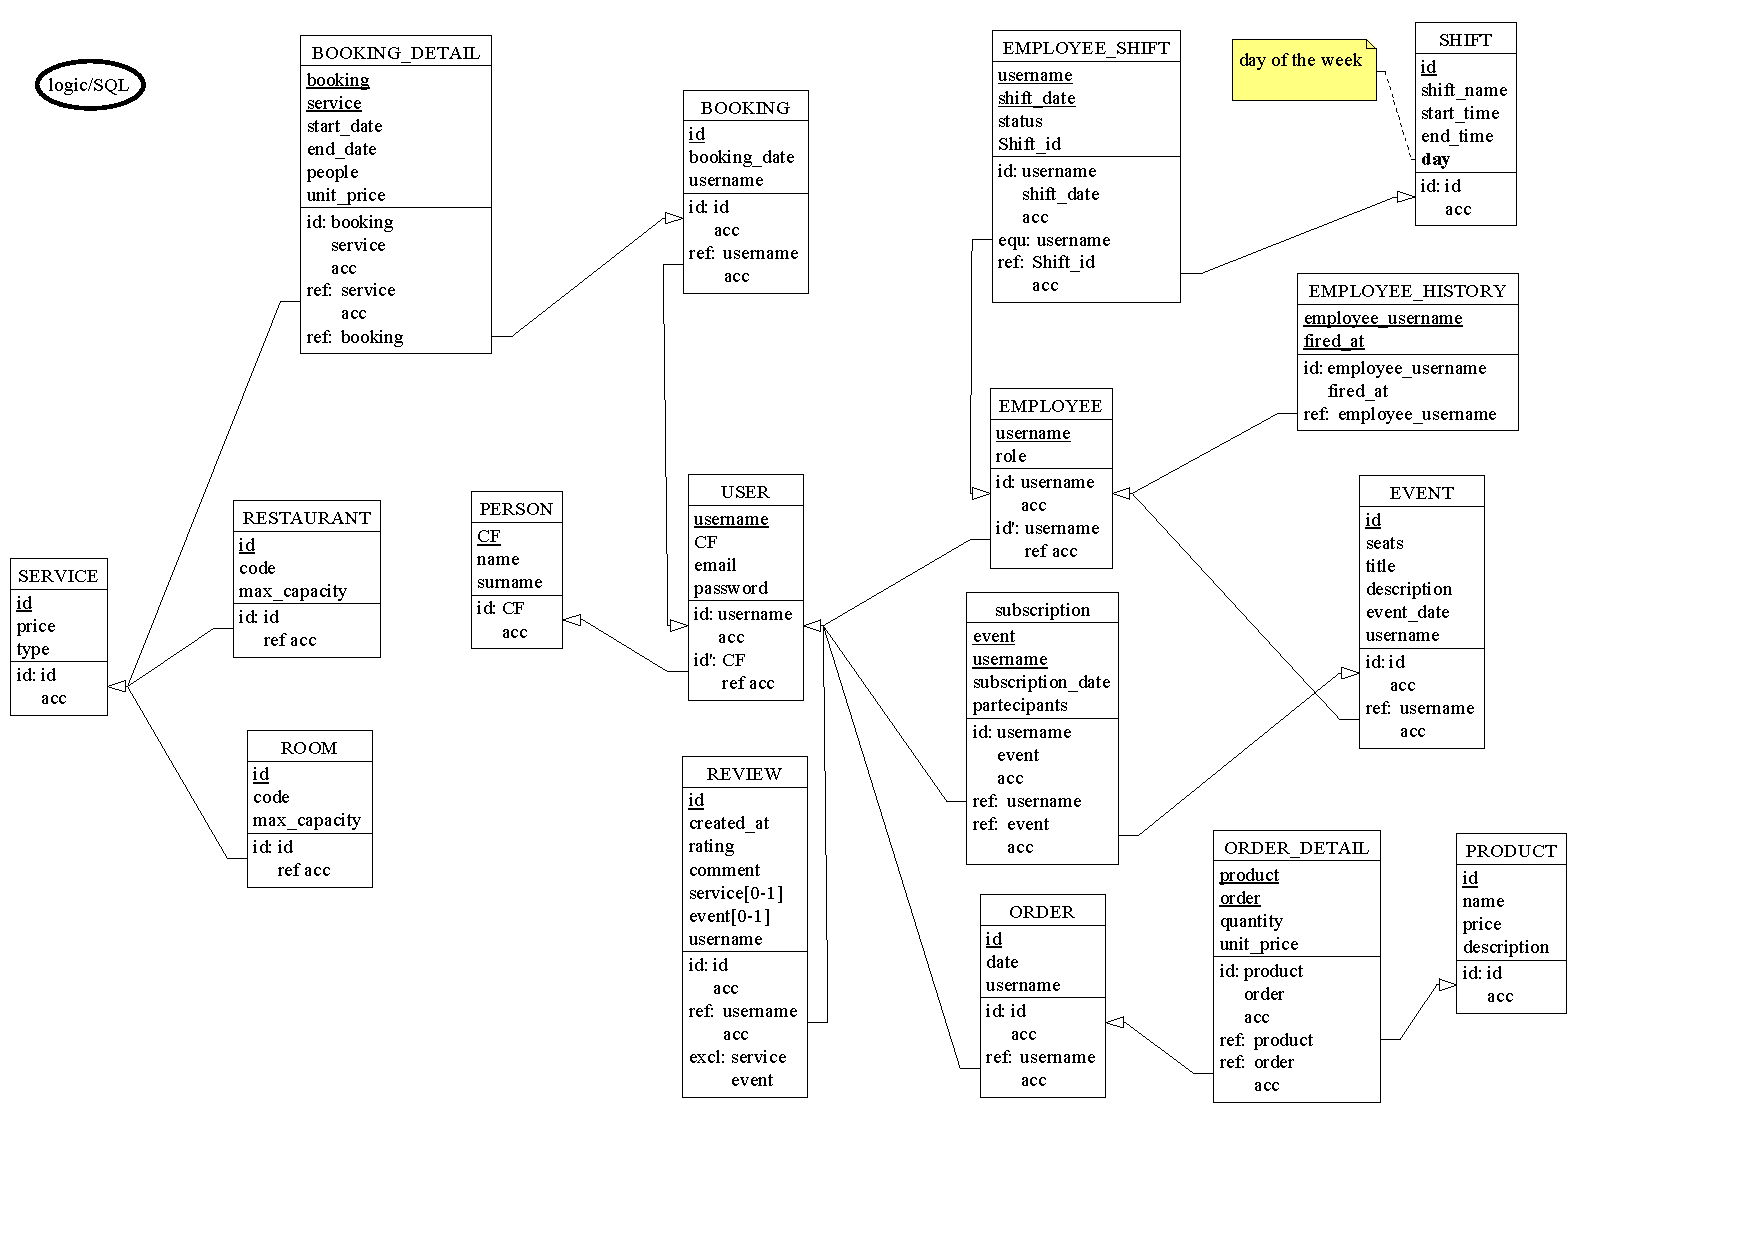
\includegraphics[width=\textwidth, trim=0 0 0 0]{./schemas/logic.pdf}
    \caption{Schema relazione finale}
    \label{fig:schema-relazione}
\end{figure}
\newpage

\chapter{Progettazione della Base di Dati}
Una volta creato il nostro database, riportiamo di seguito una parte del codice relazionale 
utilizzato per la sua implementazione.

\section{Check}
Sono stati utilizzati vincoli di tipo \texttt{CHECK} per definire alcuni domini e assicurare 
semplici proprietà degli attributi. Di seguito un esempio di vincolo \texttt{CHECK} utilizzato 
per assicurare che il prezzo di ogni prodotto sia maggiore zero:
\begin{sqlcode}[caption={},label={lst:check}]
CREATE TABLE PRODUCT (
    id INT AUTO_INCREMENT PRIMARY KEY,
    name VARCHAR(100) NOT NULL,
    description TEXT NOT NULL,
    price DECIMAL(8,2) NOT NULL CHECK (price > 0)
);
\end{sqlcode}

\section{Viste}
La seguente vista \texttt{active\_employees} restituisce l'elenco dei dipendenti attivi, 
mostrando per ciascuno username, email, nome, cognome e ruolo. Un dipendente è considerato 
attivo se il suo username non compare nella tabella \texttt{EMPLOYEE\_HISTORY}, che traccia 
lo storico delle variazioni di stato.

\begin{sqlcode}[caption={},label={lst:view}]
CREATE VIEW active_employees AS
SELECT 
    e.username,
    u.email,
    p.name,
    p.surname,
    e.role
FROM EMPLOYEE e
JOIN USER u ON e.username = u.username
JOIN PERSON p ON u.cf = p.cf
WHERE e.username NOT IN (
    SELECT username FROM EMPLOYEE_HISTORY
);
\end{sqlcode}

\section{Trigger}
Esempio di trigger per vincolare le recensioni: impedisce di recensire sia evento che servizio 
insieme, e consente la recensione solo se l'utente ha partecipato all'evento (già svolto) o ha 
usufruito del servizio.

\begin{sqlcode}[caption={},label={lst:trigger}]
DROP TRIGGER IF EXISTS trg_review_before_insert;
DELIMITER $$
CREATE TRIGGER trg_review_before_insert
BEFORE INSERT ON REVIEW
FOR EACH ROW
BEGIN
    DECLARE cnt INT DEFAULT 0;

    IF (NEW.event IS NOT NULL AND NEW.service IS NOT NULL) OR (NEW.event IS NULL AND NEW.service IS NULL) THEN
        SIGNAL SQLSTATE '45000'
            SET MESSAGE_TEXT = 'Set either event or service (not both) for the review.';
    END IF;

    IF NEW.event IS NOT NULL THEN
        SELECT COUNT(*)
            INTO cnt
            FROM EVENT e
            JOIN EVENT_SUBSCRIPTION es
                ON es.event = e.id
             AND es.`user` = NEW.`user`
         WHERE e.id = NEW.event
             AND e.event_date < CURDATE();

        IF cnt = 0 THEN
            SIGNAL SQLSTATE '45000'
                SET MESSAGE_TEXT = 'You can review the event only if you were subscribed and the event date is in the past.';
        END IF;
    END IF;

    IF NEW.service IS NOT NULL THEN
        SELECT COUNT(*)
            INTO cnt
            FROM RESERVATION r
            JOIN RESERVATION_DETAIL rd
                ON rd.reservation = r.id
             AND rd.service = NEW.service
         WHERE r.username = NEW.`user`
             AND rd.end_date < NOW();

        IF cnt = 0 THEN
            SIGNAL SQLSTATE '45000'
                SET MESSAGE_TEXT = 'You can review the service only after you have used it (completed reservation).';
        END IF;
    END IF;
END$$
DELIMITER ;
\end{sqlcode}

\section{Traduzione delle operazioni}

\chapter{Progettazione dell'applicazione}
L'applicazione è stata sviluppata con il framework \textbf{Django}, che gestisce routing, 
database e autenticazione in modo sicuro e scalabile.

\section{Barra di Navigazione}
La \textbf{barra di navigazione} permette un accesso rapido alle principali sezioni del sito, 
come prodotti, eventi, servizi, area personale e funzioni amministrative.

\begin{figure}[H]
    \centering
    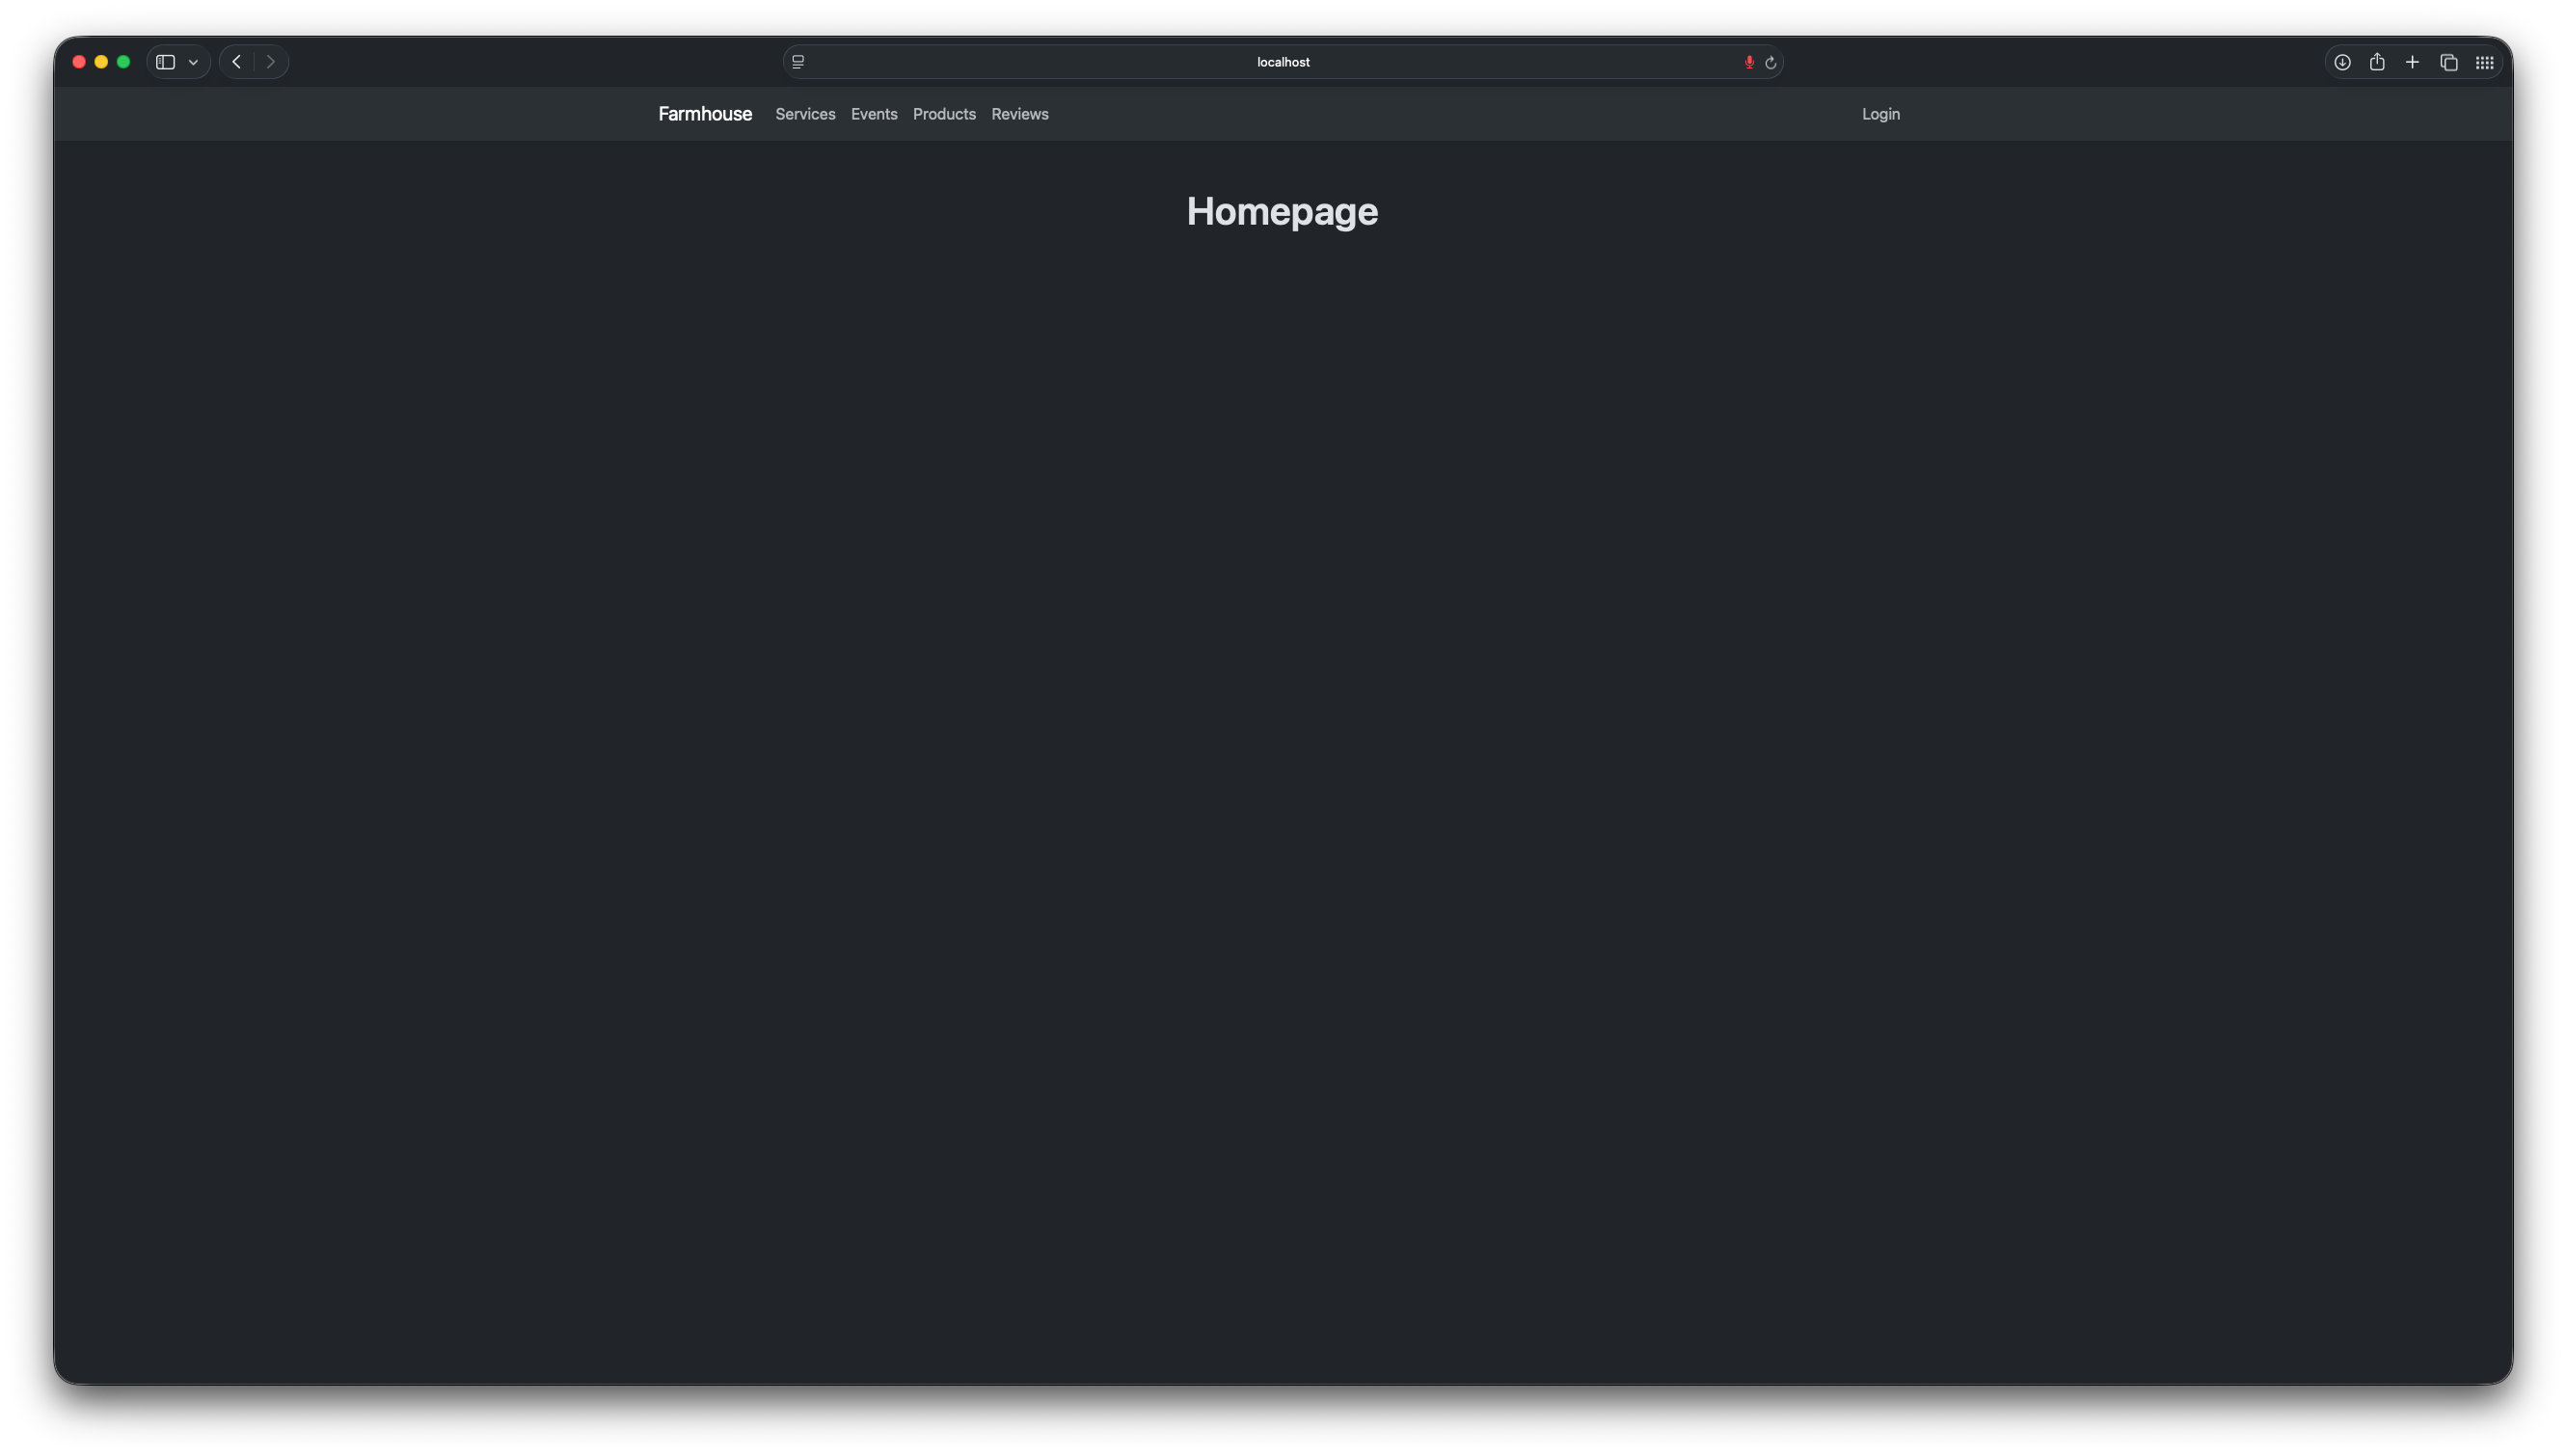
\includegraphics[width=\textwidth, trim=0 0 0 0]{./img/navbar.png}
    \caption{Barra di navigazione}
    \label{fig:navbar}
\end{figure}

\newpage
\subsection*{Login}

Il form di login consente agli utenti registrati di accedere rapidamente alla piattaforma inserendo username e 
password. Il sistema verifica le credenziali e, in caso di errore, mostra un messaggio di avviso.

\begin{figure}[H]
    \centering
    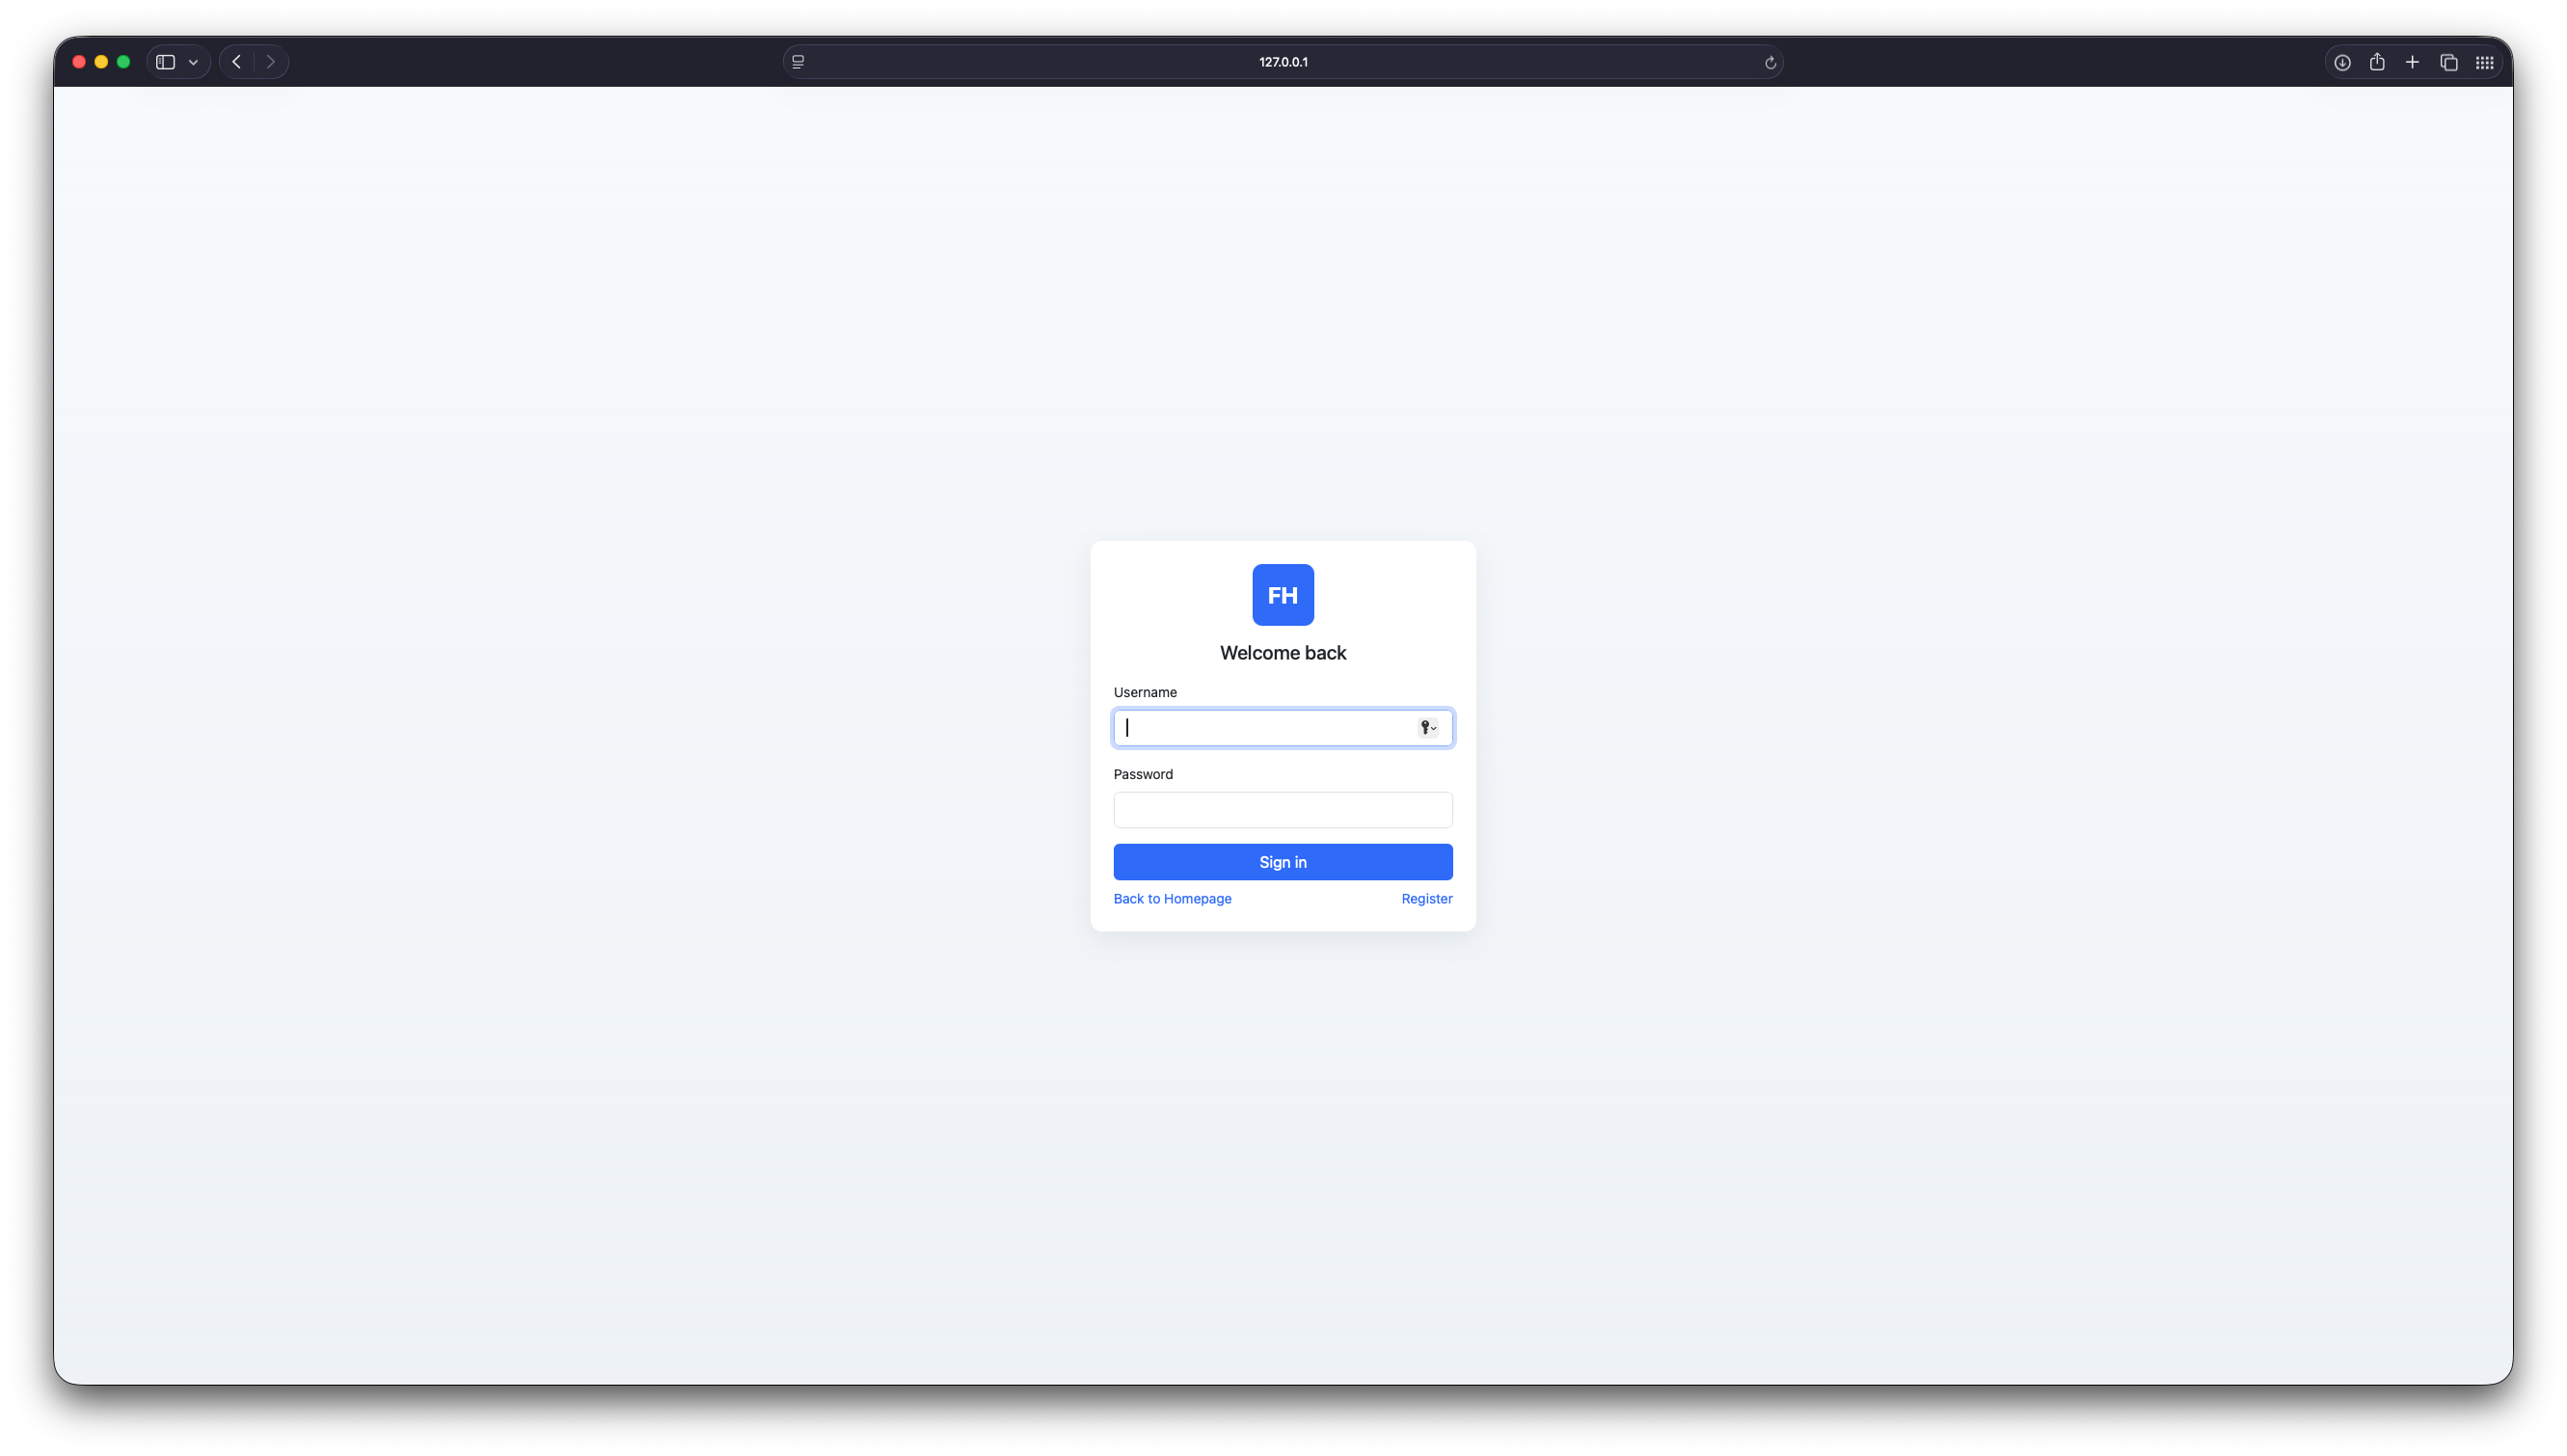
\includegraphics[width=\textwidth, trim=0 0 0 0]{./img/login.png}
    \vspace{-1em}
    \label{fig:login}
\end{figure}

\subsection*{Registrazione}
Anche per registrarsi è disponibile un form semplice e intuitivo, che permette agli utenti di creare un nuovo 
account inserendo i dati richiesti. Dopo la registrazione, l'utente potrà accedere a tutte le funzionalità della 
piattaforma.

\begin{figure}[H]
    \centering
    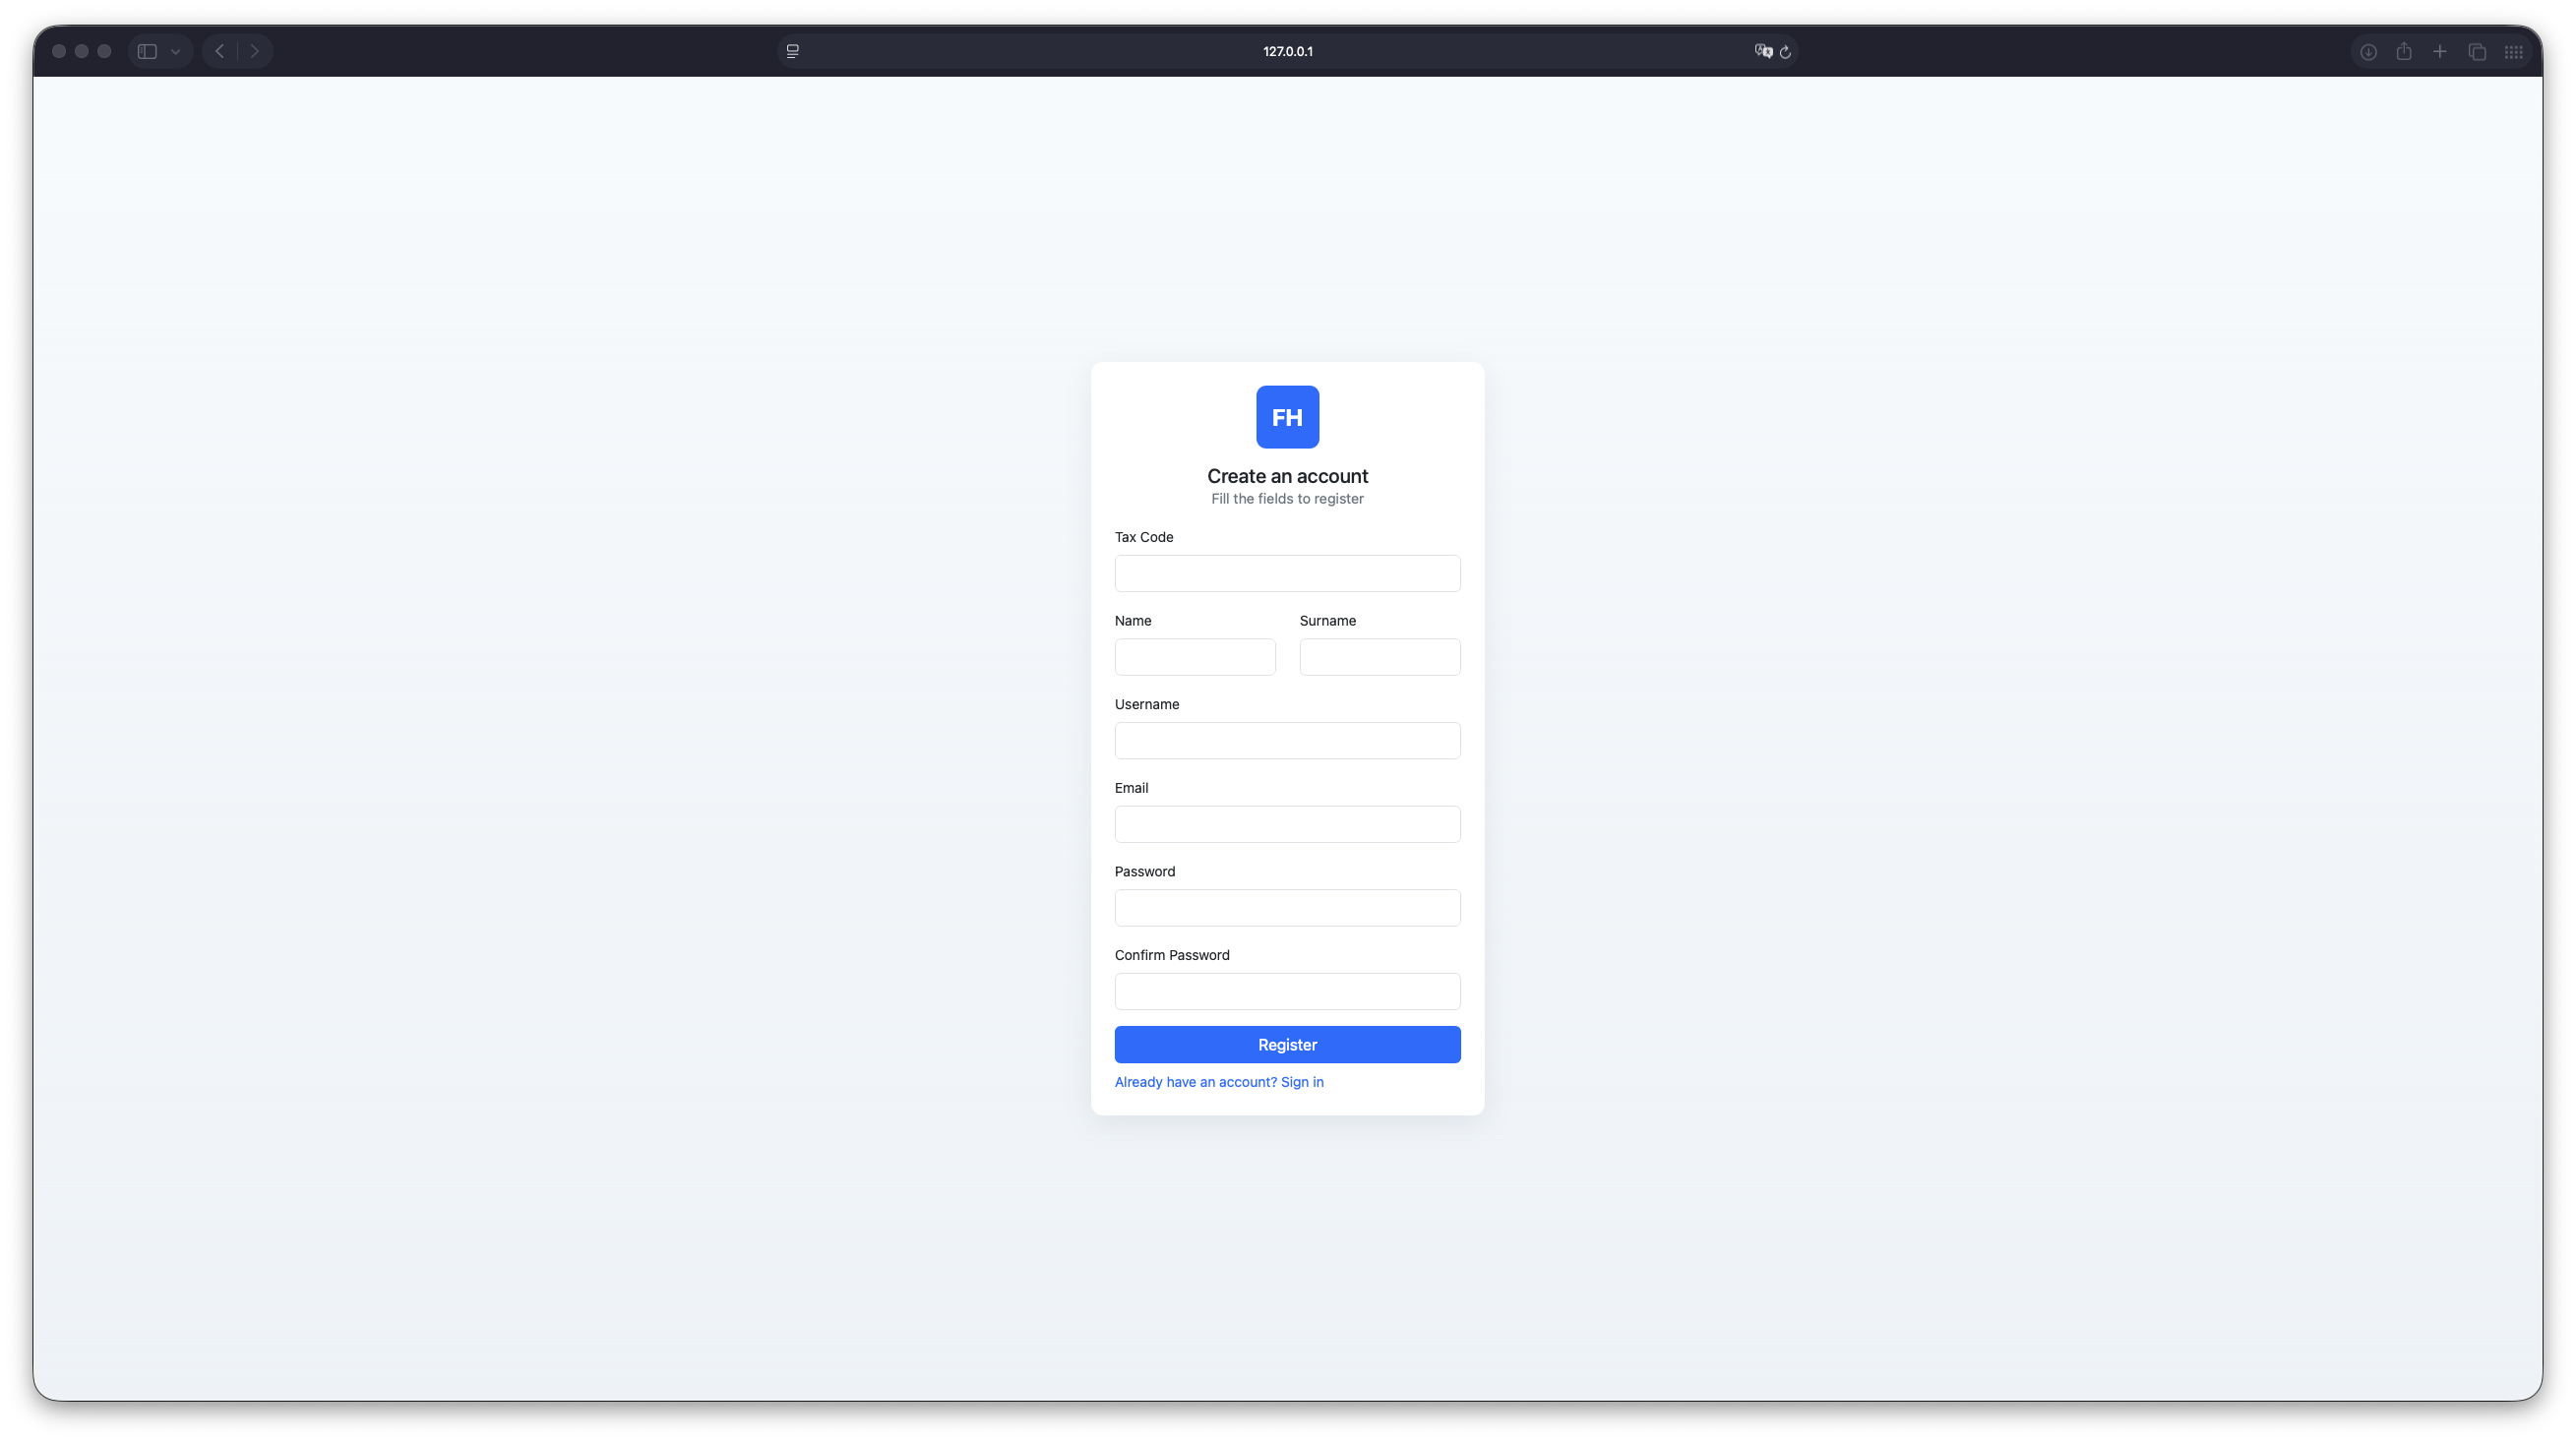
\includegraphics[width=\textwidth, trim=0 0 0 0]{./img/register.png}
    \vspace{-1em}
    \label{fig:registrazione}
\end{figure}

\newpage
\section{Interfaccia Utente}
Dopo l'accesso, l'utente potrà visualizzare il profilo, con le prenotazioni e gli ordini, con 
la possibilità di recensire o annullare prenotazioni future.

\begin{figure}[H]
    \centering
    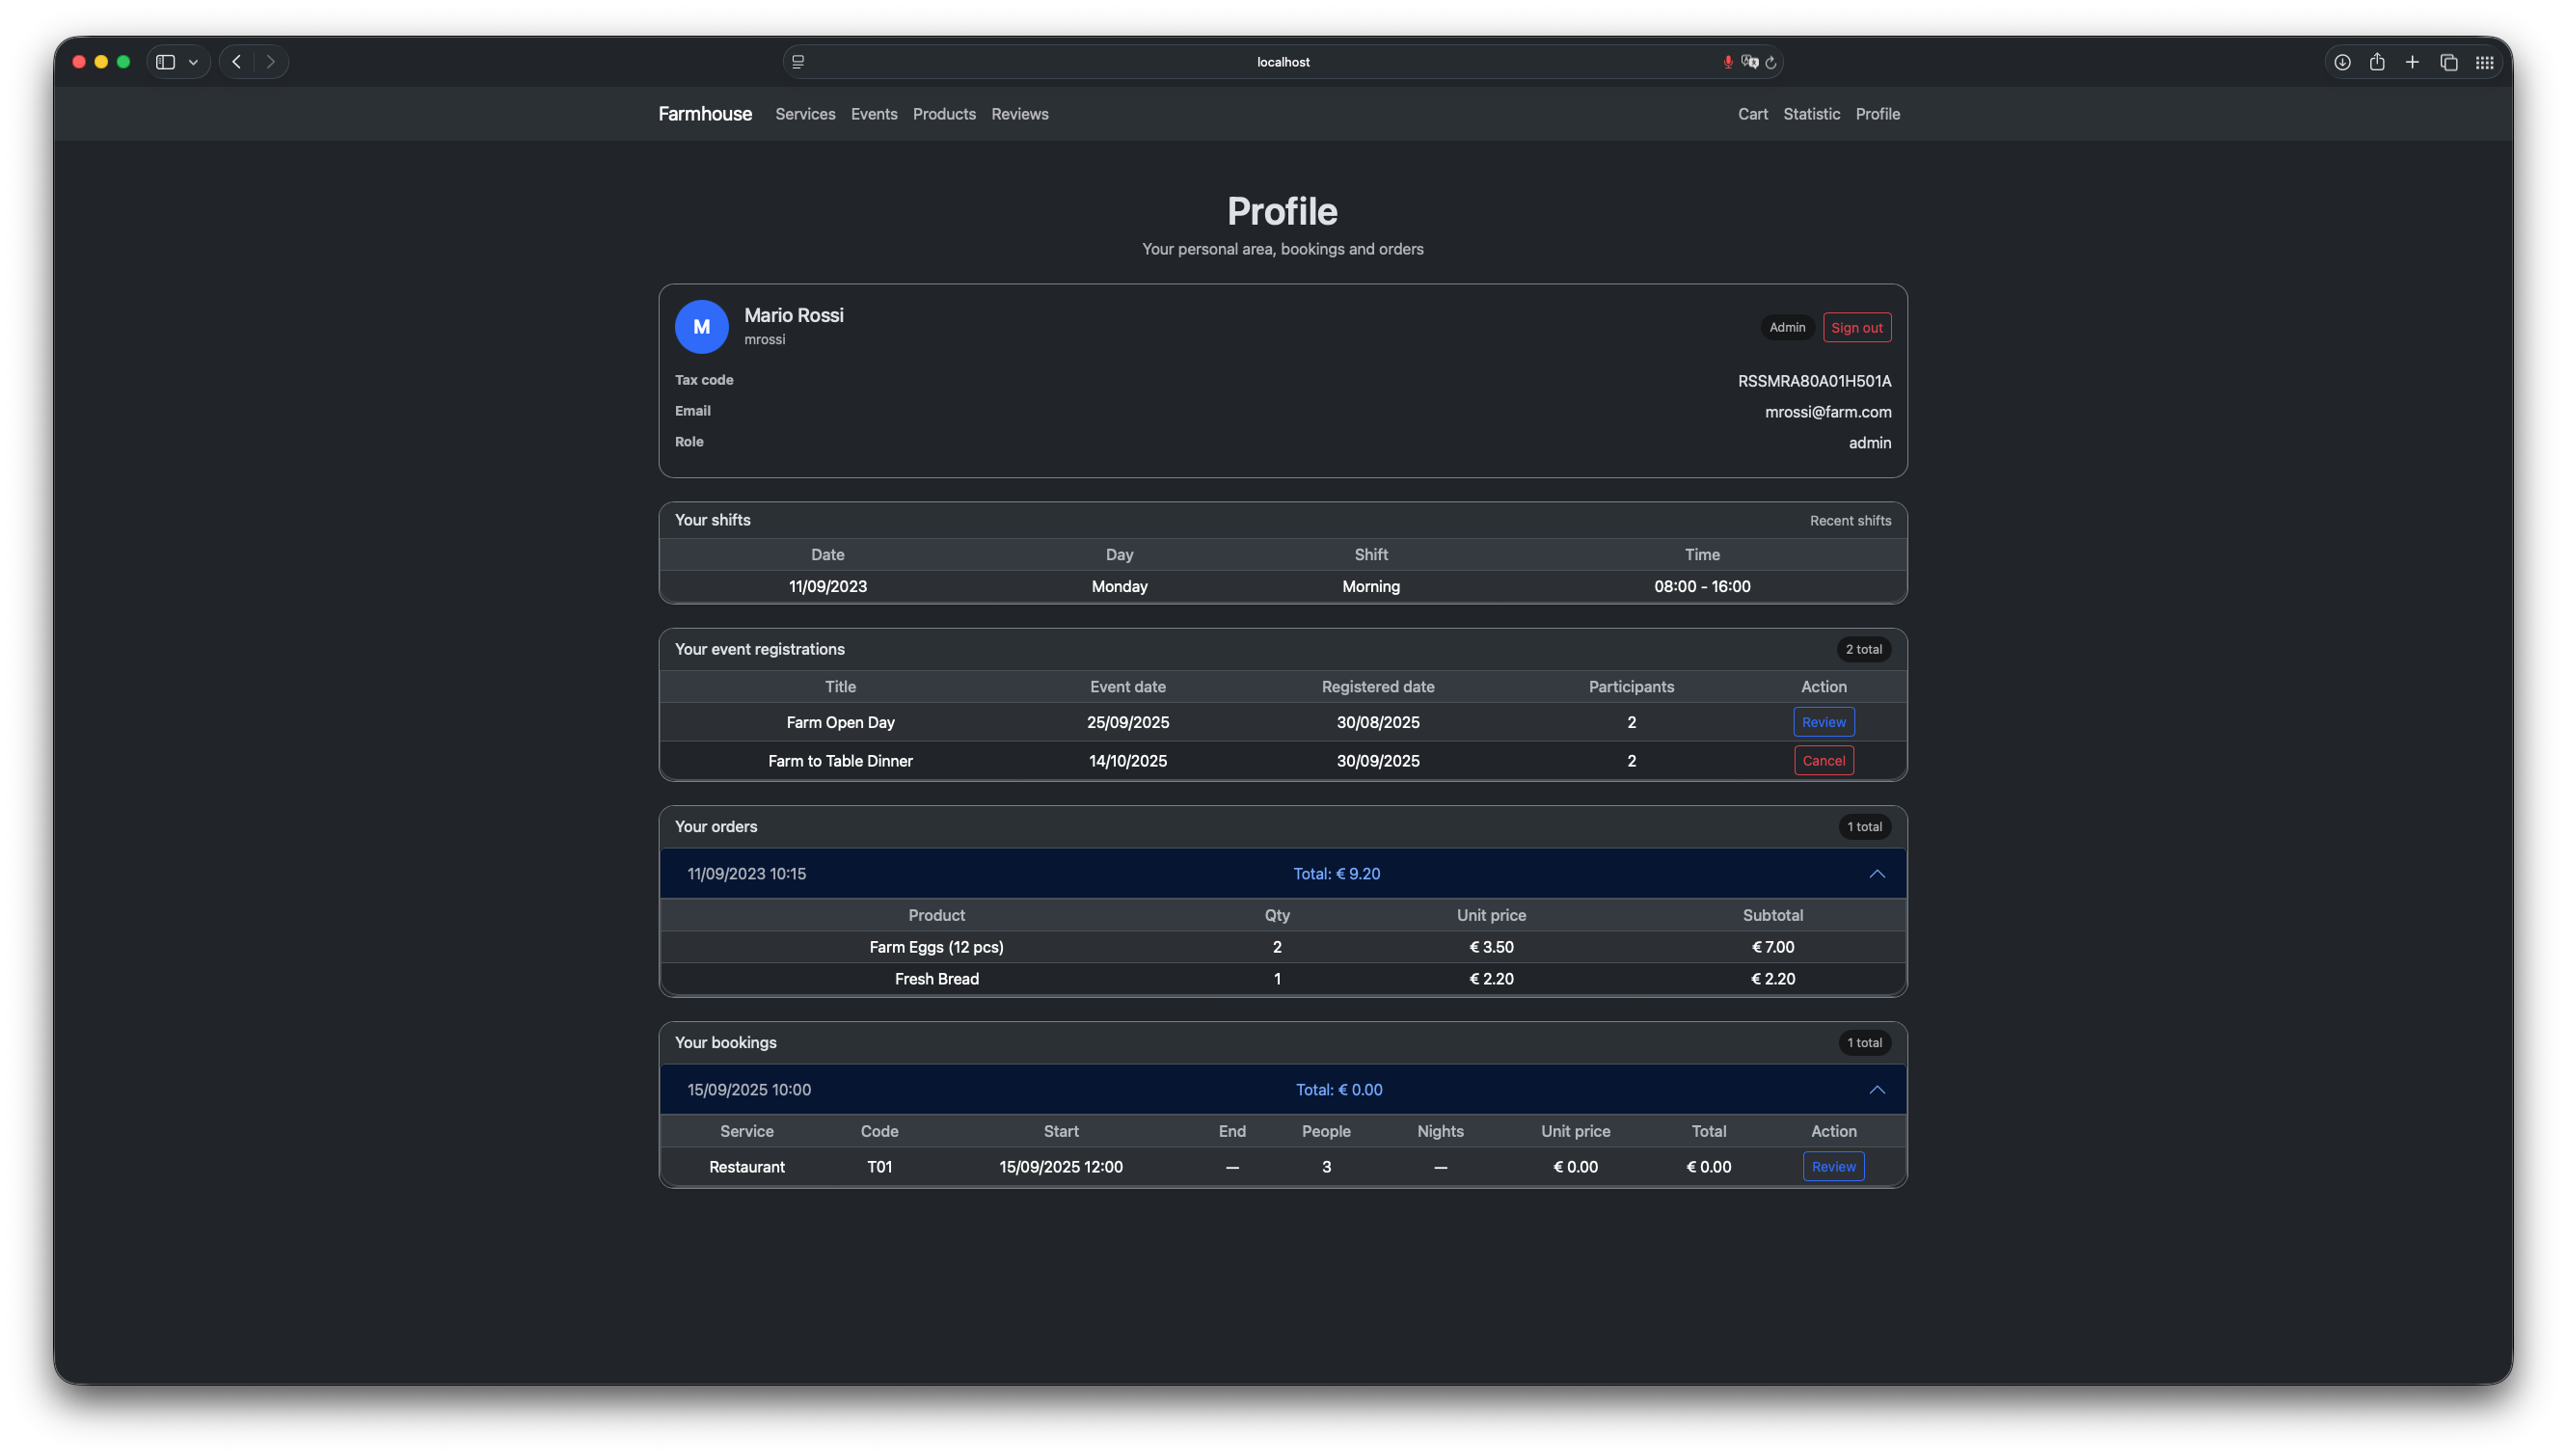
\includegraphics[width=\textwidth, trim=0 0 0 0]{./img/users/profile.png}
    \vspace{-1em}
    \label{fig:profile}
\end{figure}

\subsection*{Servizi}
Dopo aver scelto il servizio da prenotare, è sufficiente inserire i dati necessari; il sistema 
mostrerà la disponibilità aggiornata del servizio selezionato.

\begin{figure}[H]
    \centering
    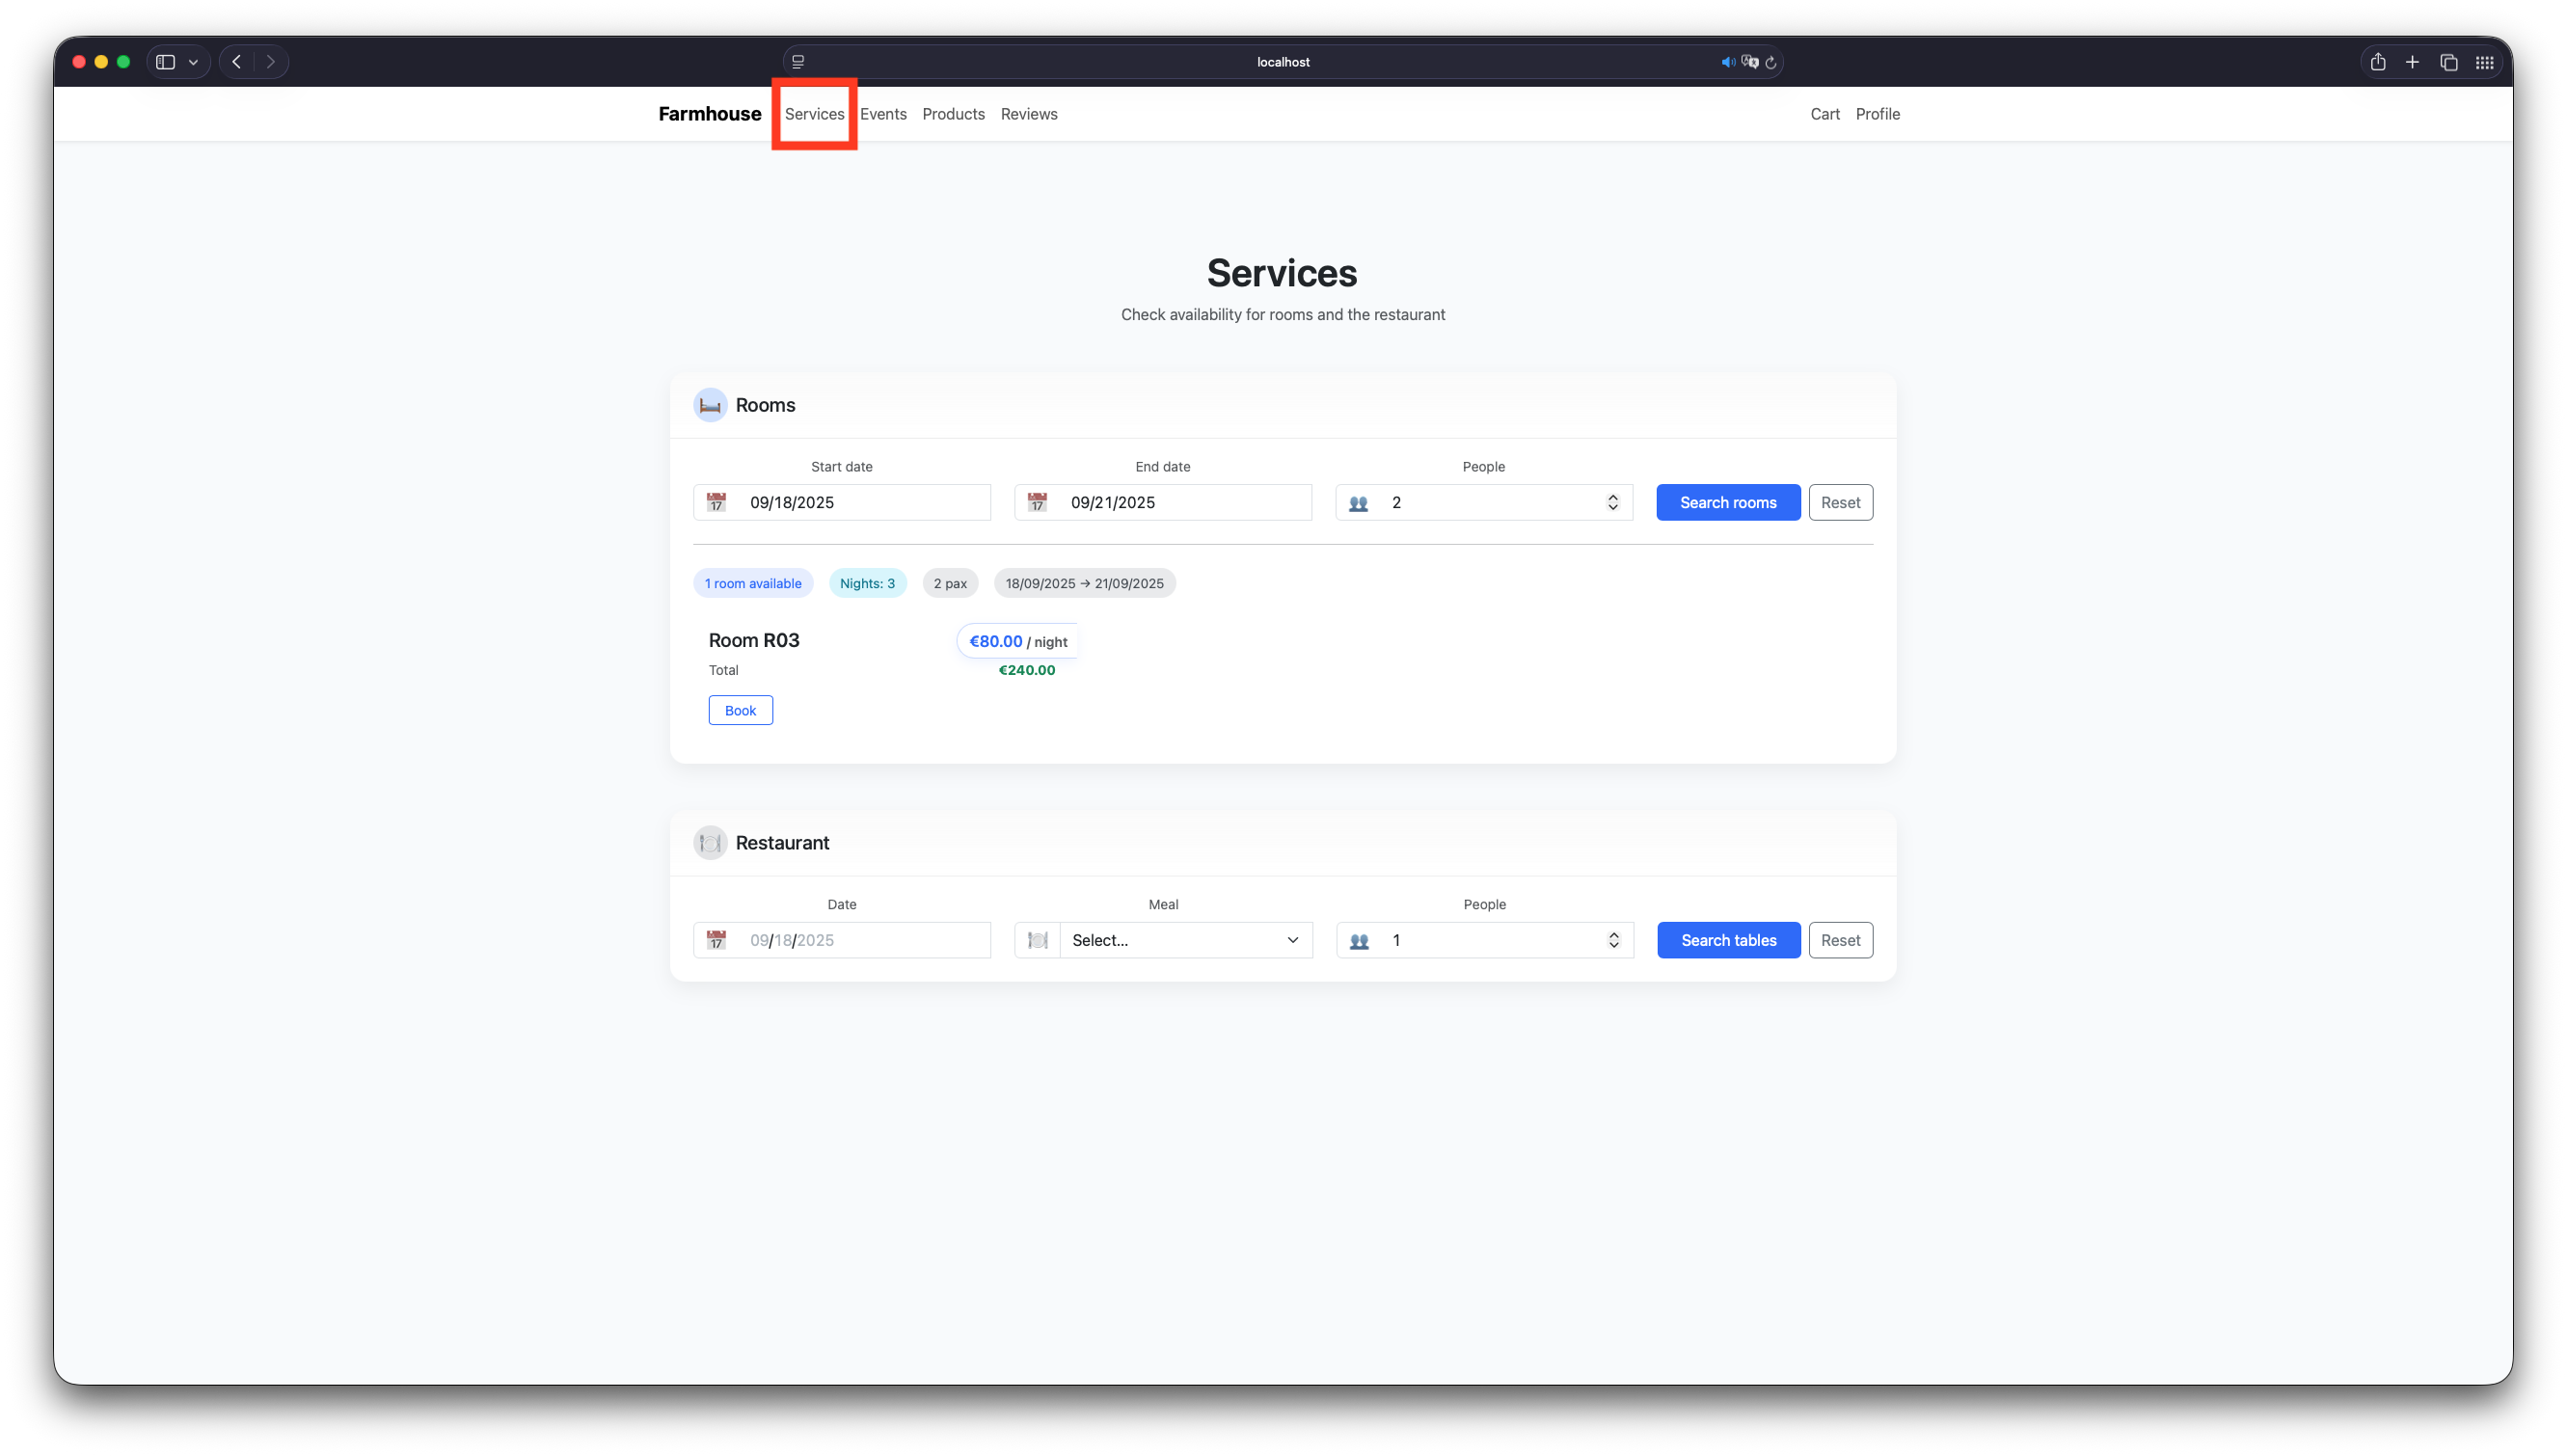
\includegraphics[width=\textwidth, trim=0 0 0 0]{./img/users/services.png}
    \vspace{-1em}
    \label{fig:services}
\end{figure}

\subsection*{Eventi}
Nella sezione eventi, viene mostrato l'elenco degli eventi disponibili. L'utente può selezionare 
l'evento di interesse, specificare il numero di partecipanti e procedere con la prenotazione. 

\begin{figure}[H]
    \centering
    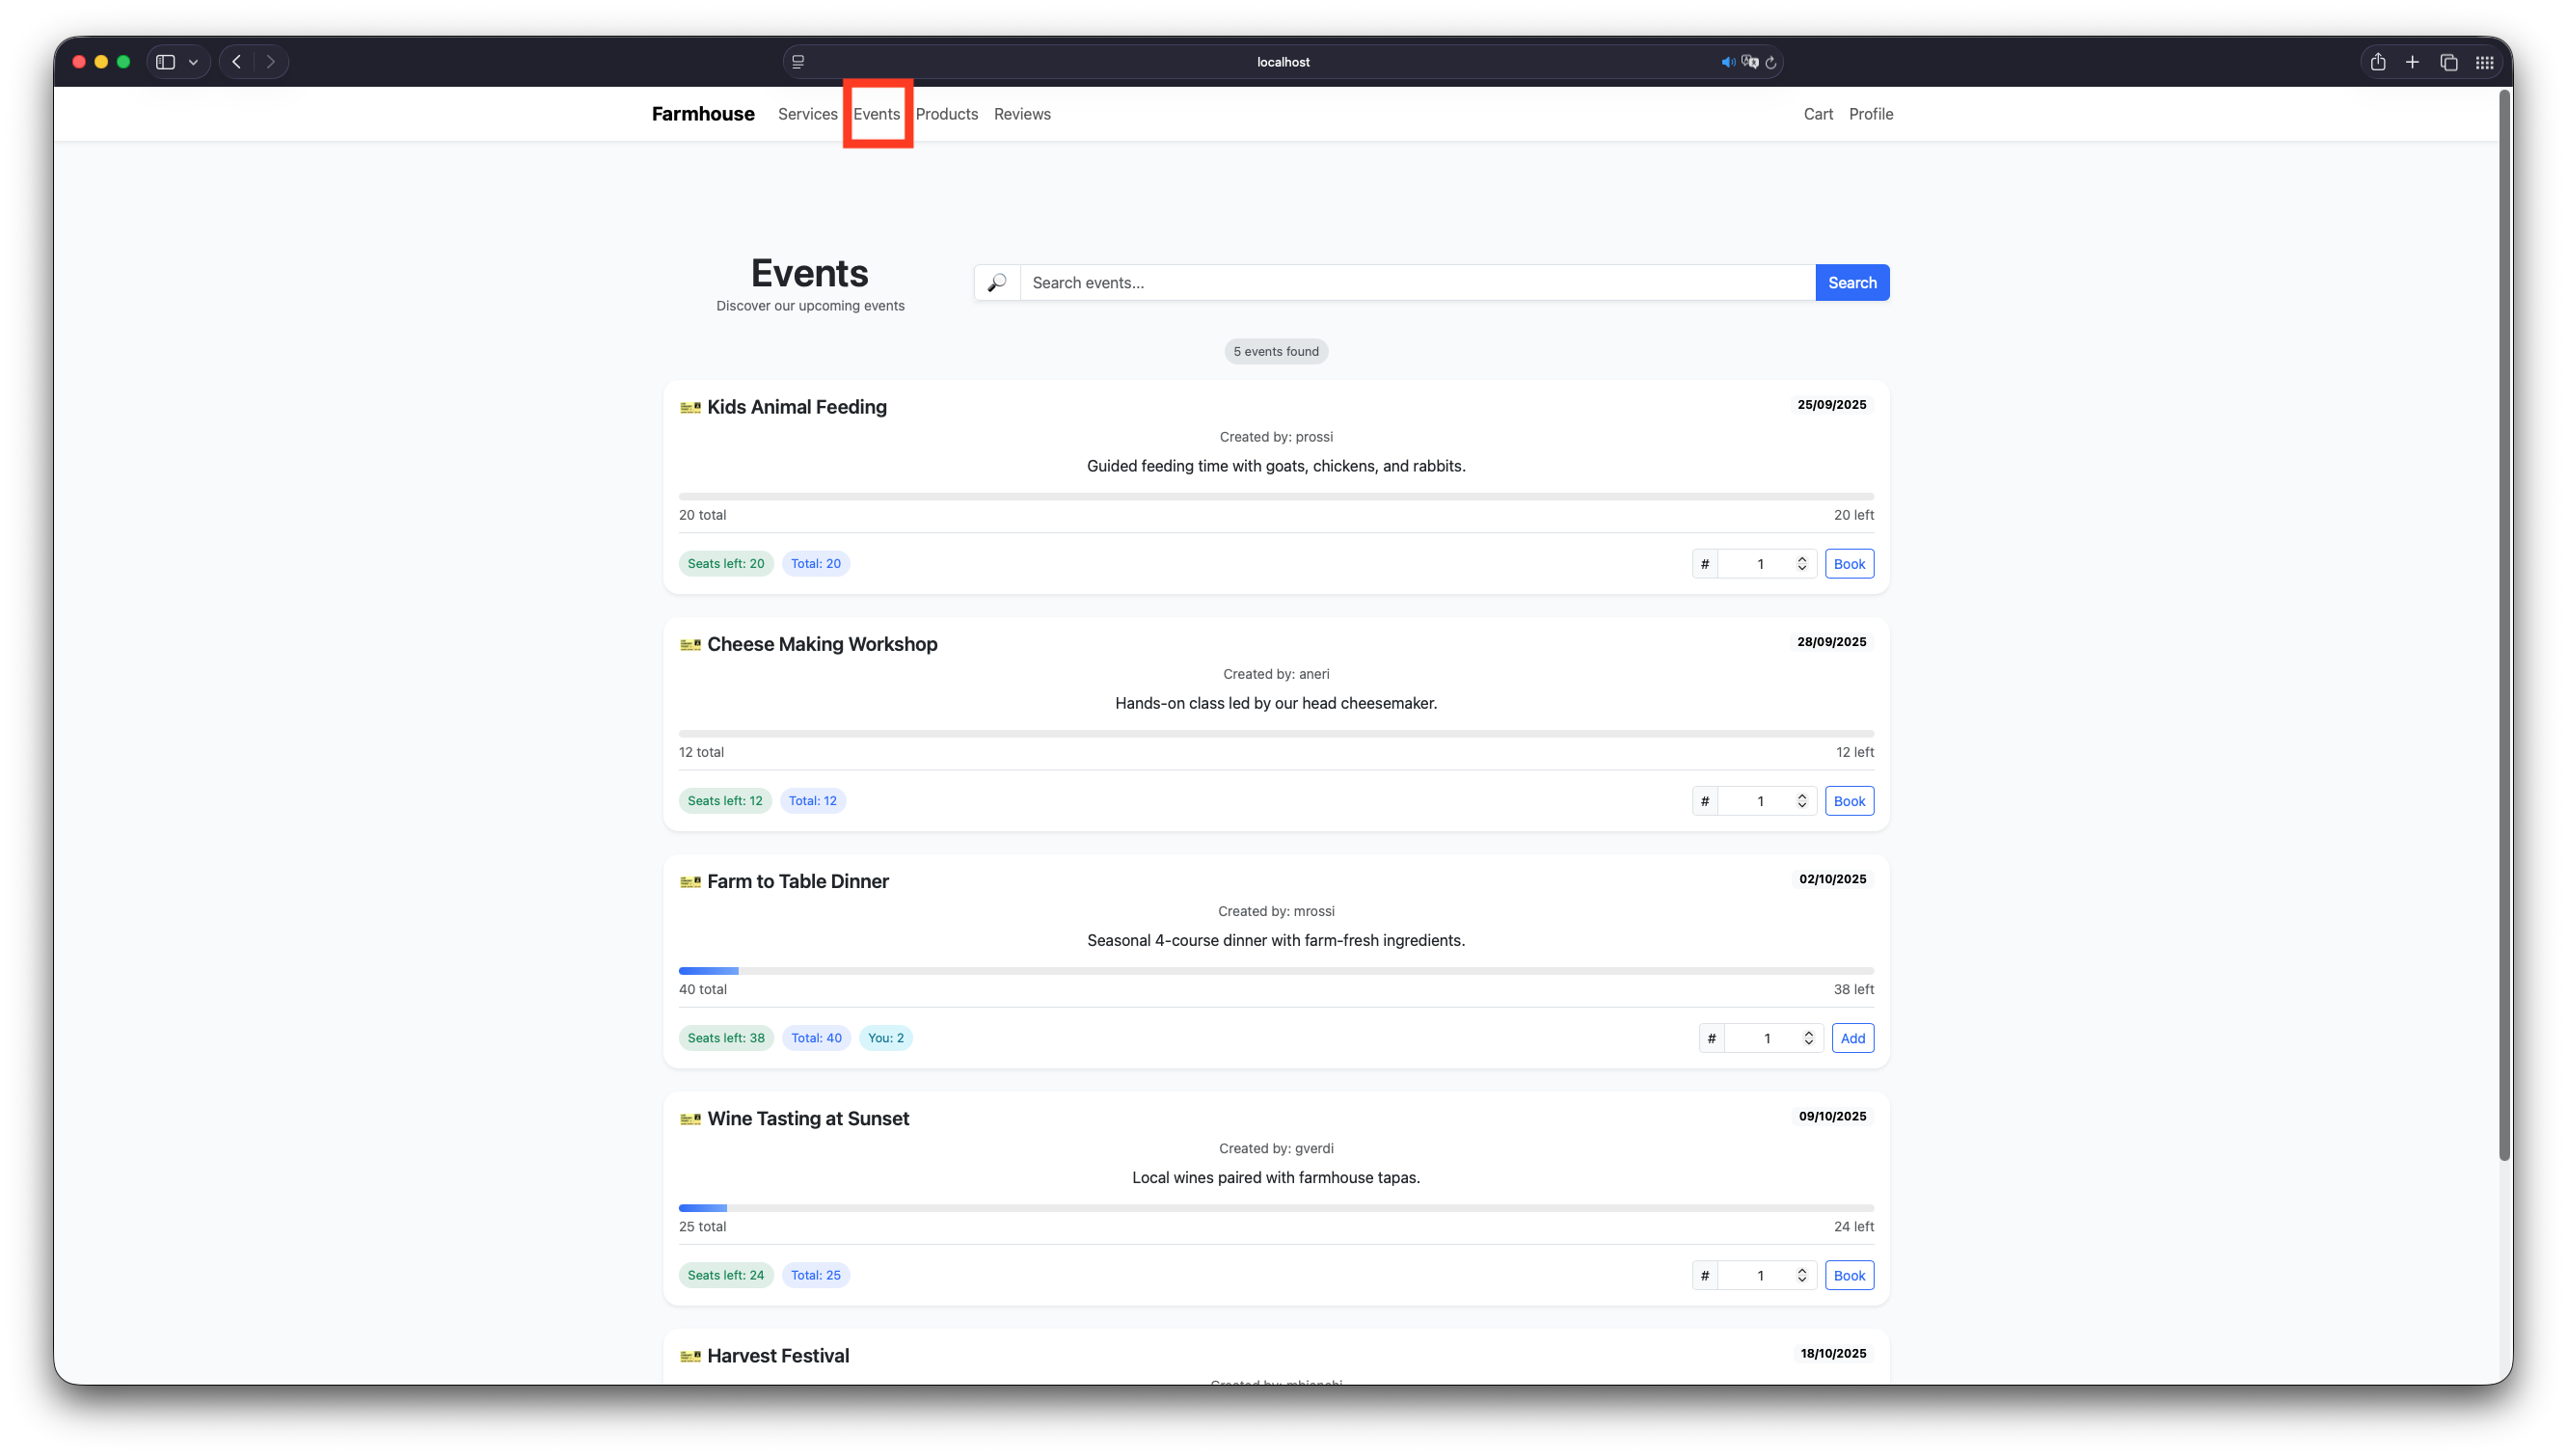
\includegraphics[width=\textwidth, trim=0 0 0 0]{./img/users/events.png}
    \vspace{-1em}
    \label{fig:events}
\end{figure}

\subsection*{Recensioni}
Gli utenti possono visualizzare tutte le recensioni e filtrarle per evento o servizio.

\begin{figure}[H]
    \centering
    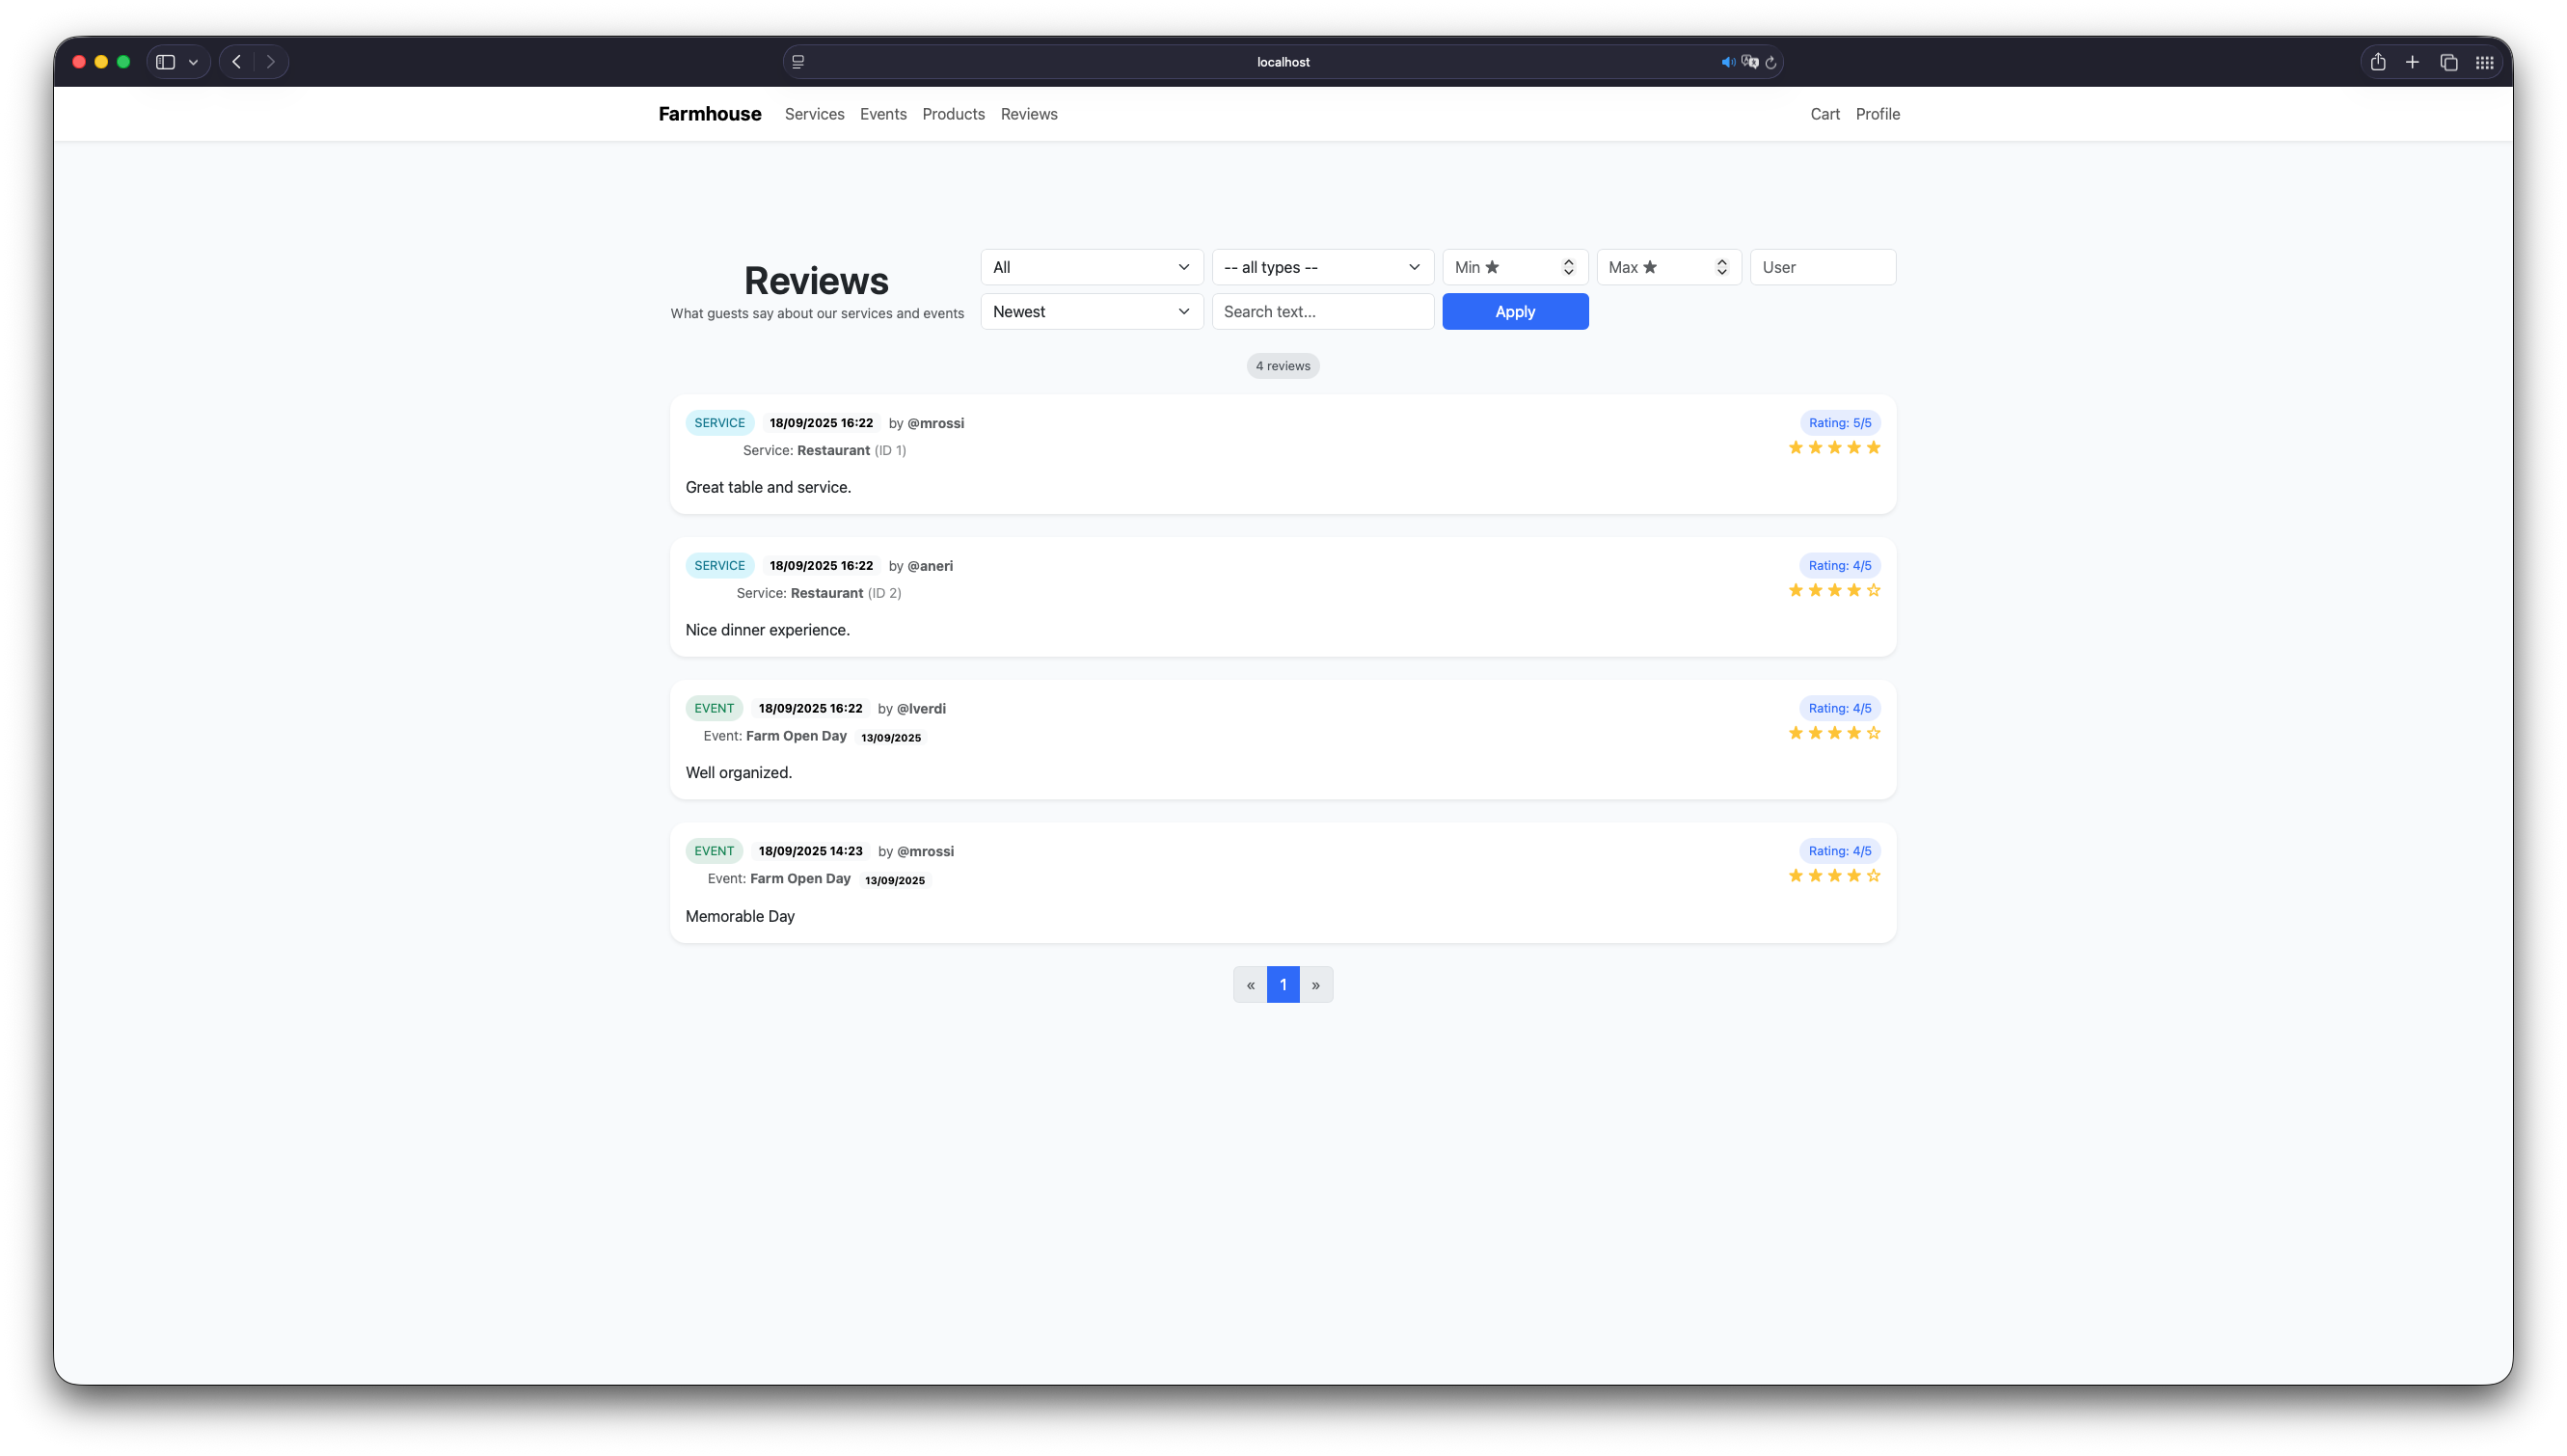
\includegraphics[width=\textwidth, trim=0 0 0 0]{./img/users/reviews.png}
    \vspace{-1em}
    \label{fig:recensione}
\end{figure}

Il form permette agli utenti di lasciare una recensione su eventi o servizi a cui hanno partecipato, 
inserendo commento e voto. La recensione è consentita solo dopo la partecipazione effettiva.

\begin{figure}[H]
    \centering
    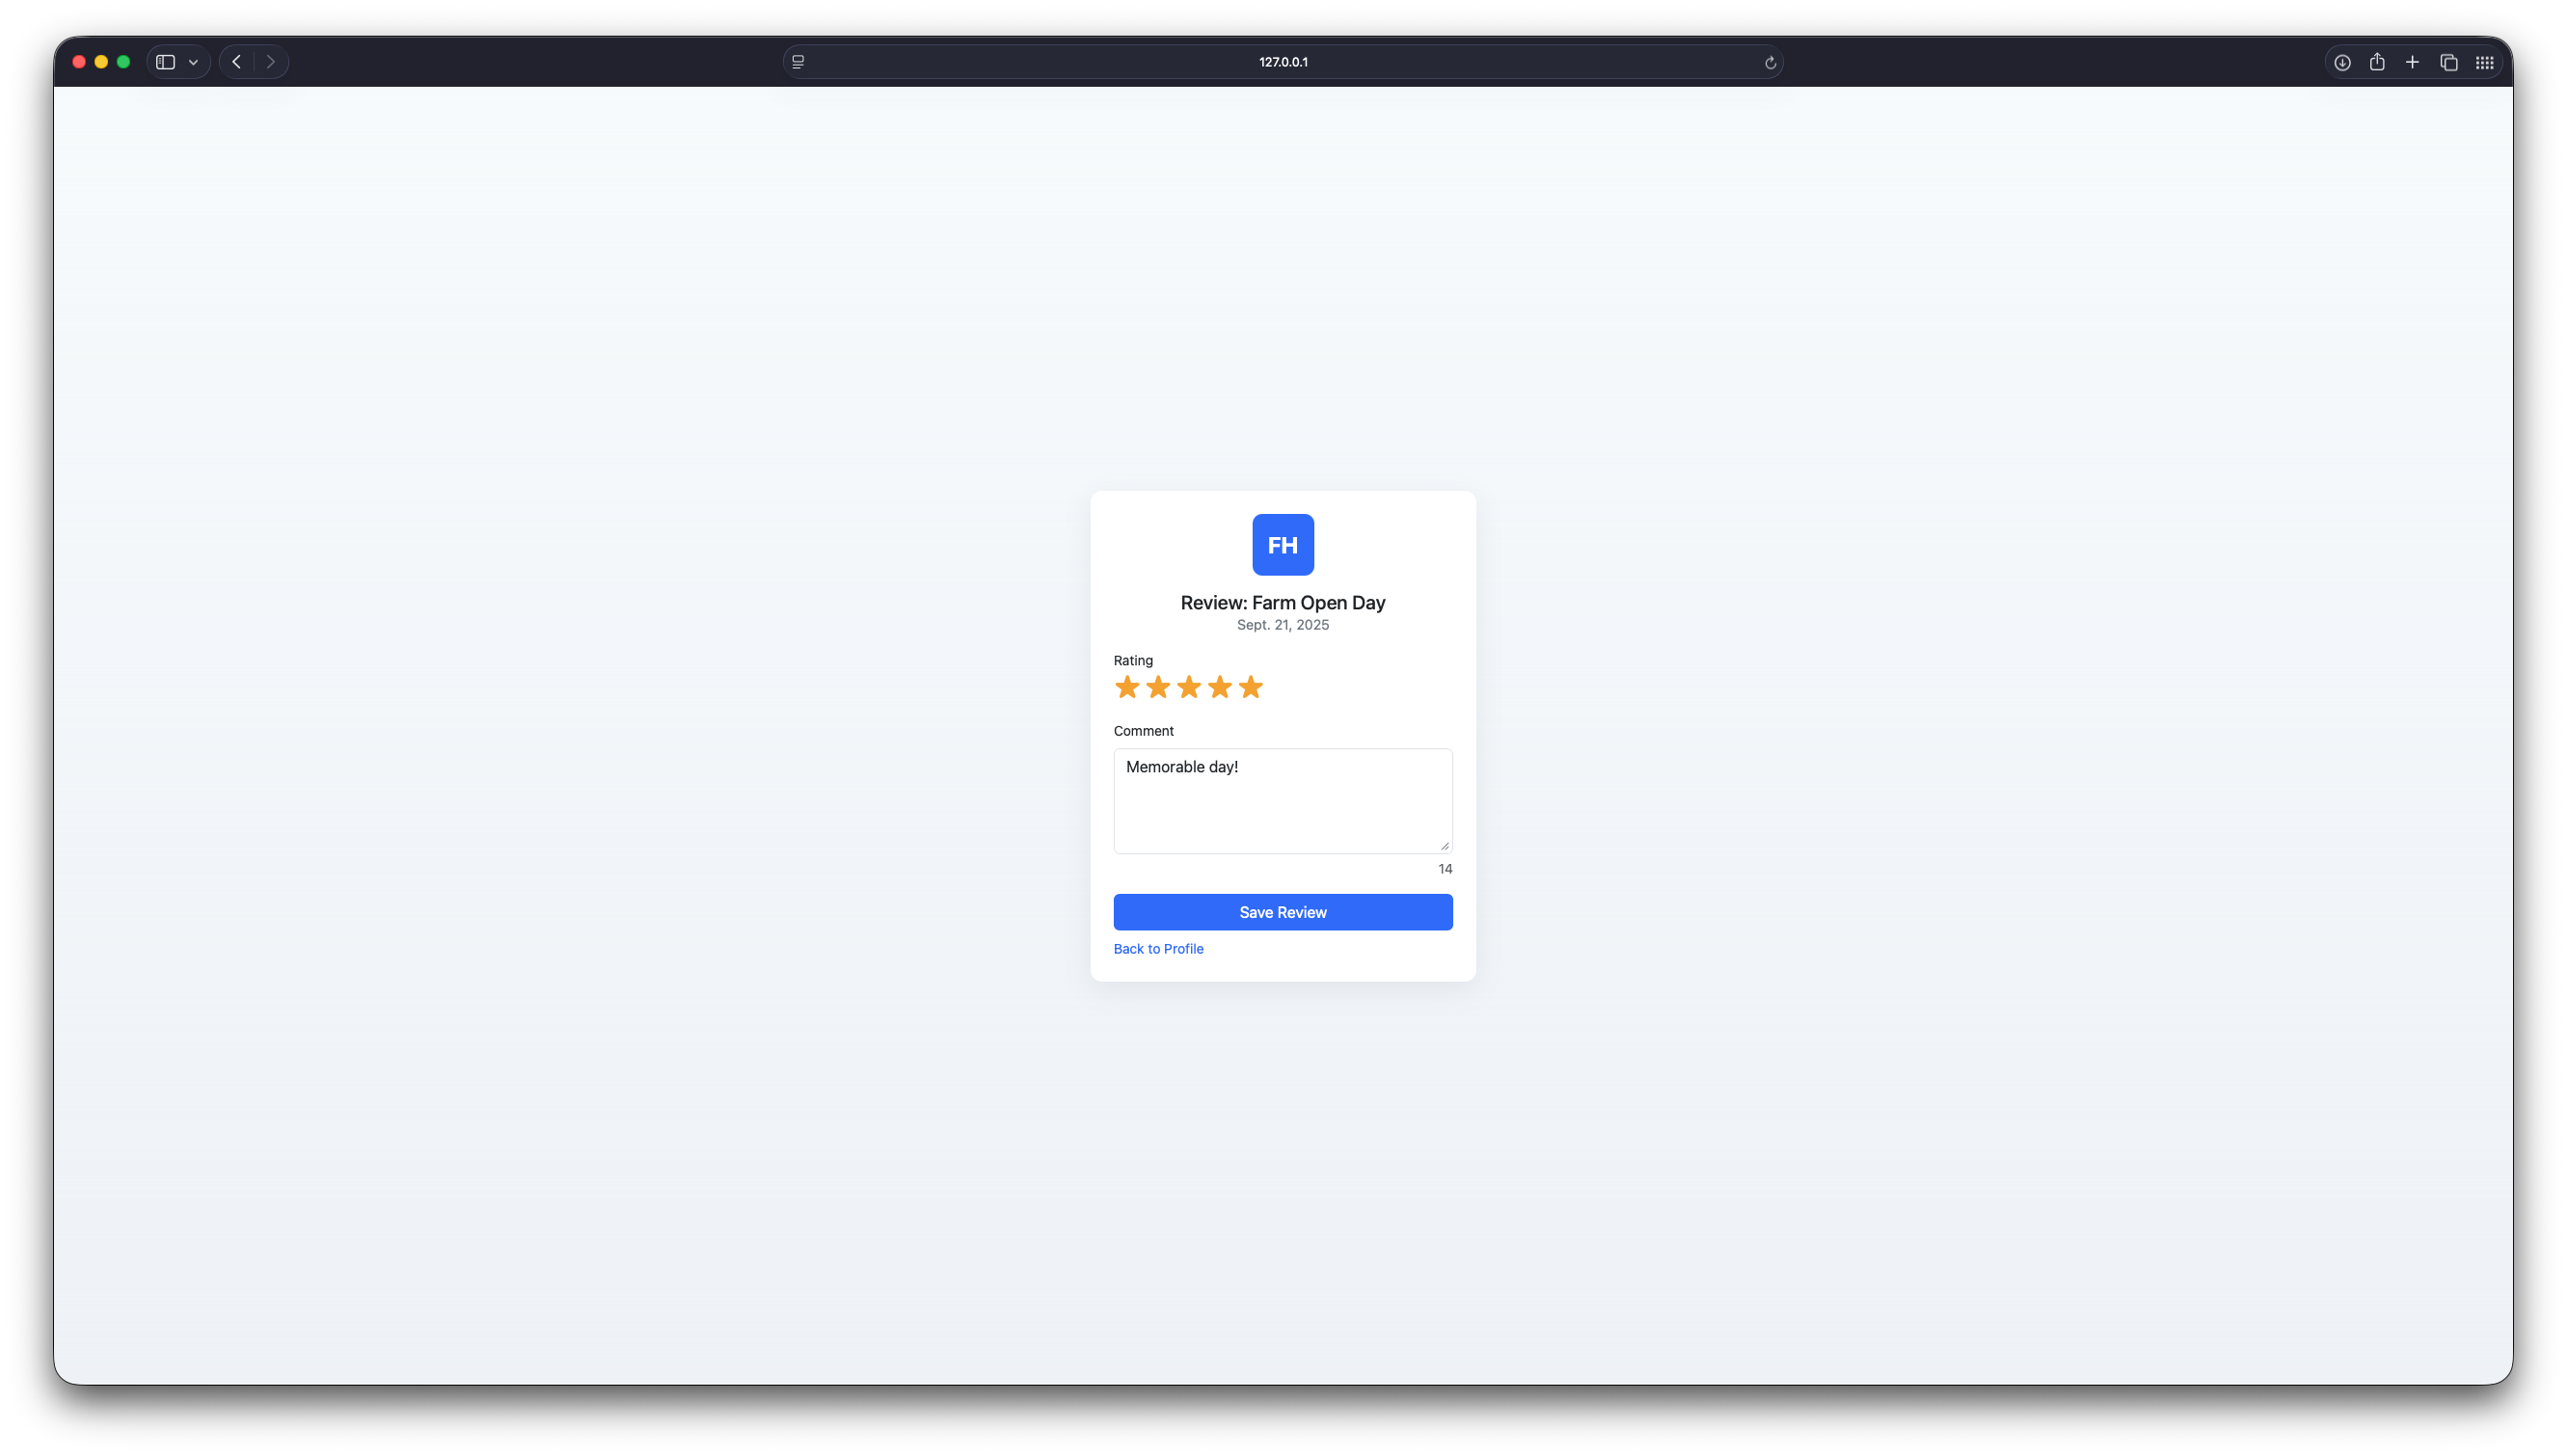
\includegraphics[width=\textwidth, trim=0 0 0 0]{./img/users/give_review.png}
    \vspace{-1em}
    \label{fig:lascia recensione}
\end{figure}

\subsection*{Prodotti}
La sezione prodotti consente agli utenti di consultare il catalogo aggiungerli al carrello per 
l'acquisto. Il sistema mostra in tempo reale il contenuto del carrello e il totale dell'ordine. 
Fatto il checkout sarà visibile il riepilogo nella sezione profilo.

\begin{figure}[H]
    \centering
    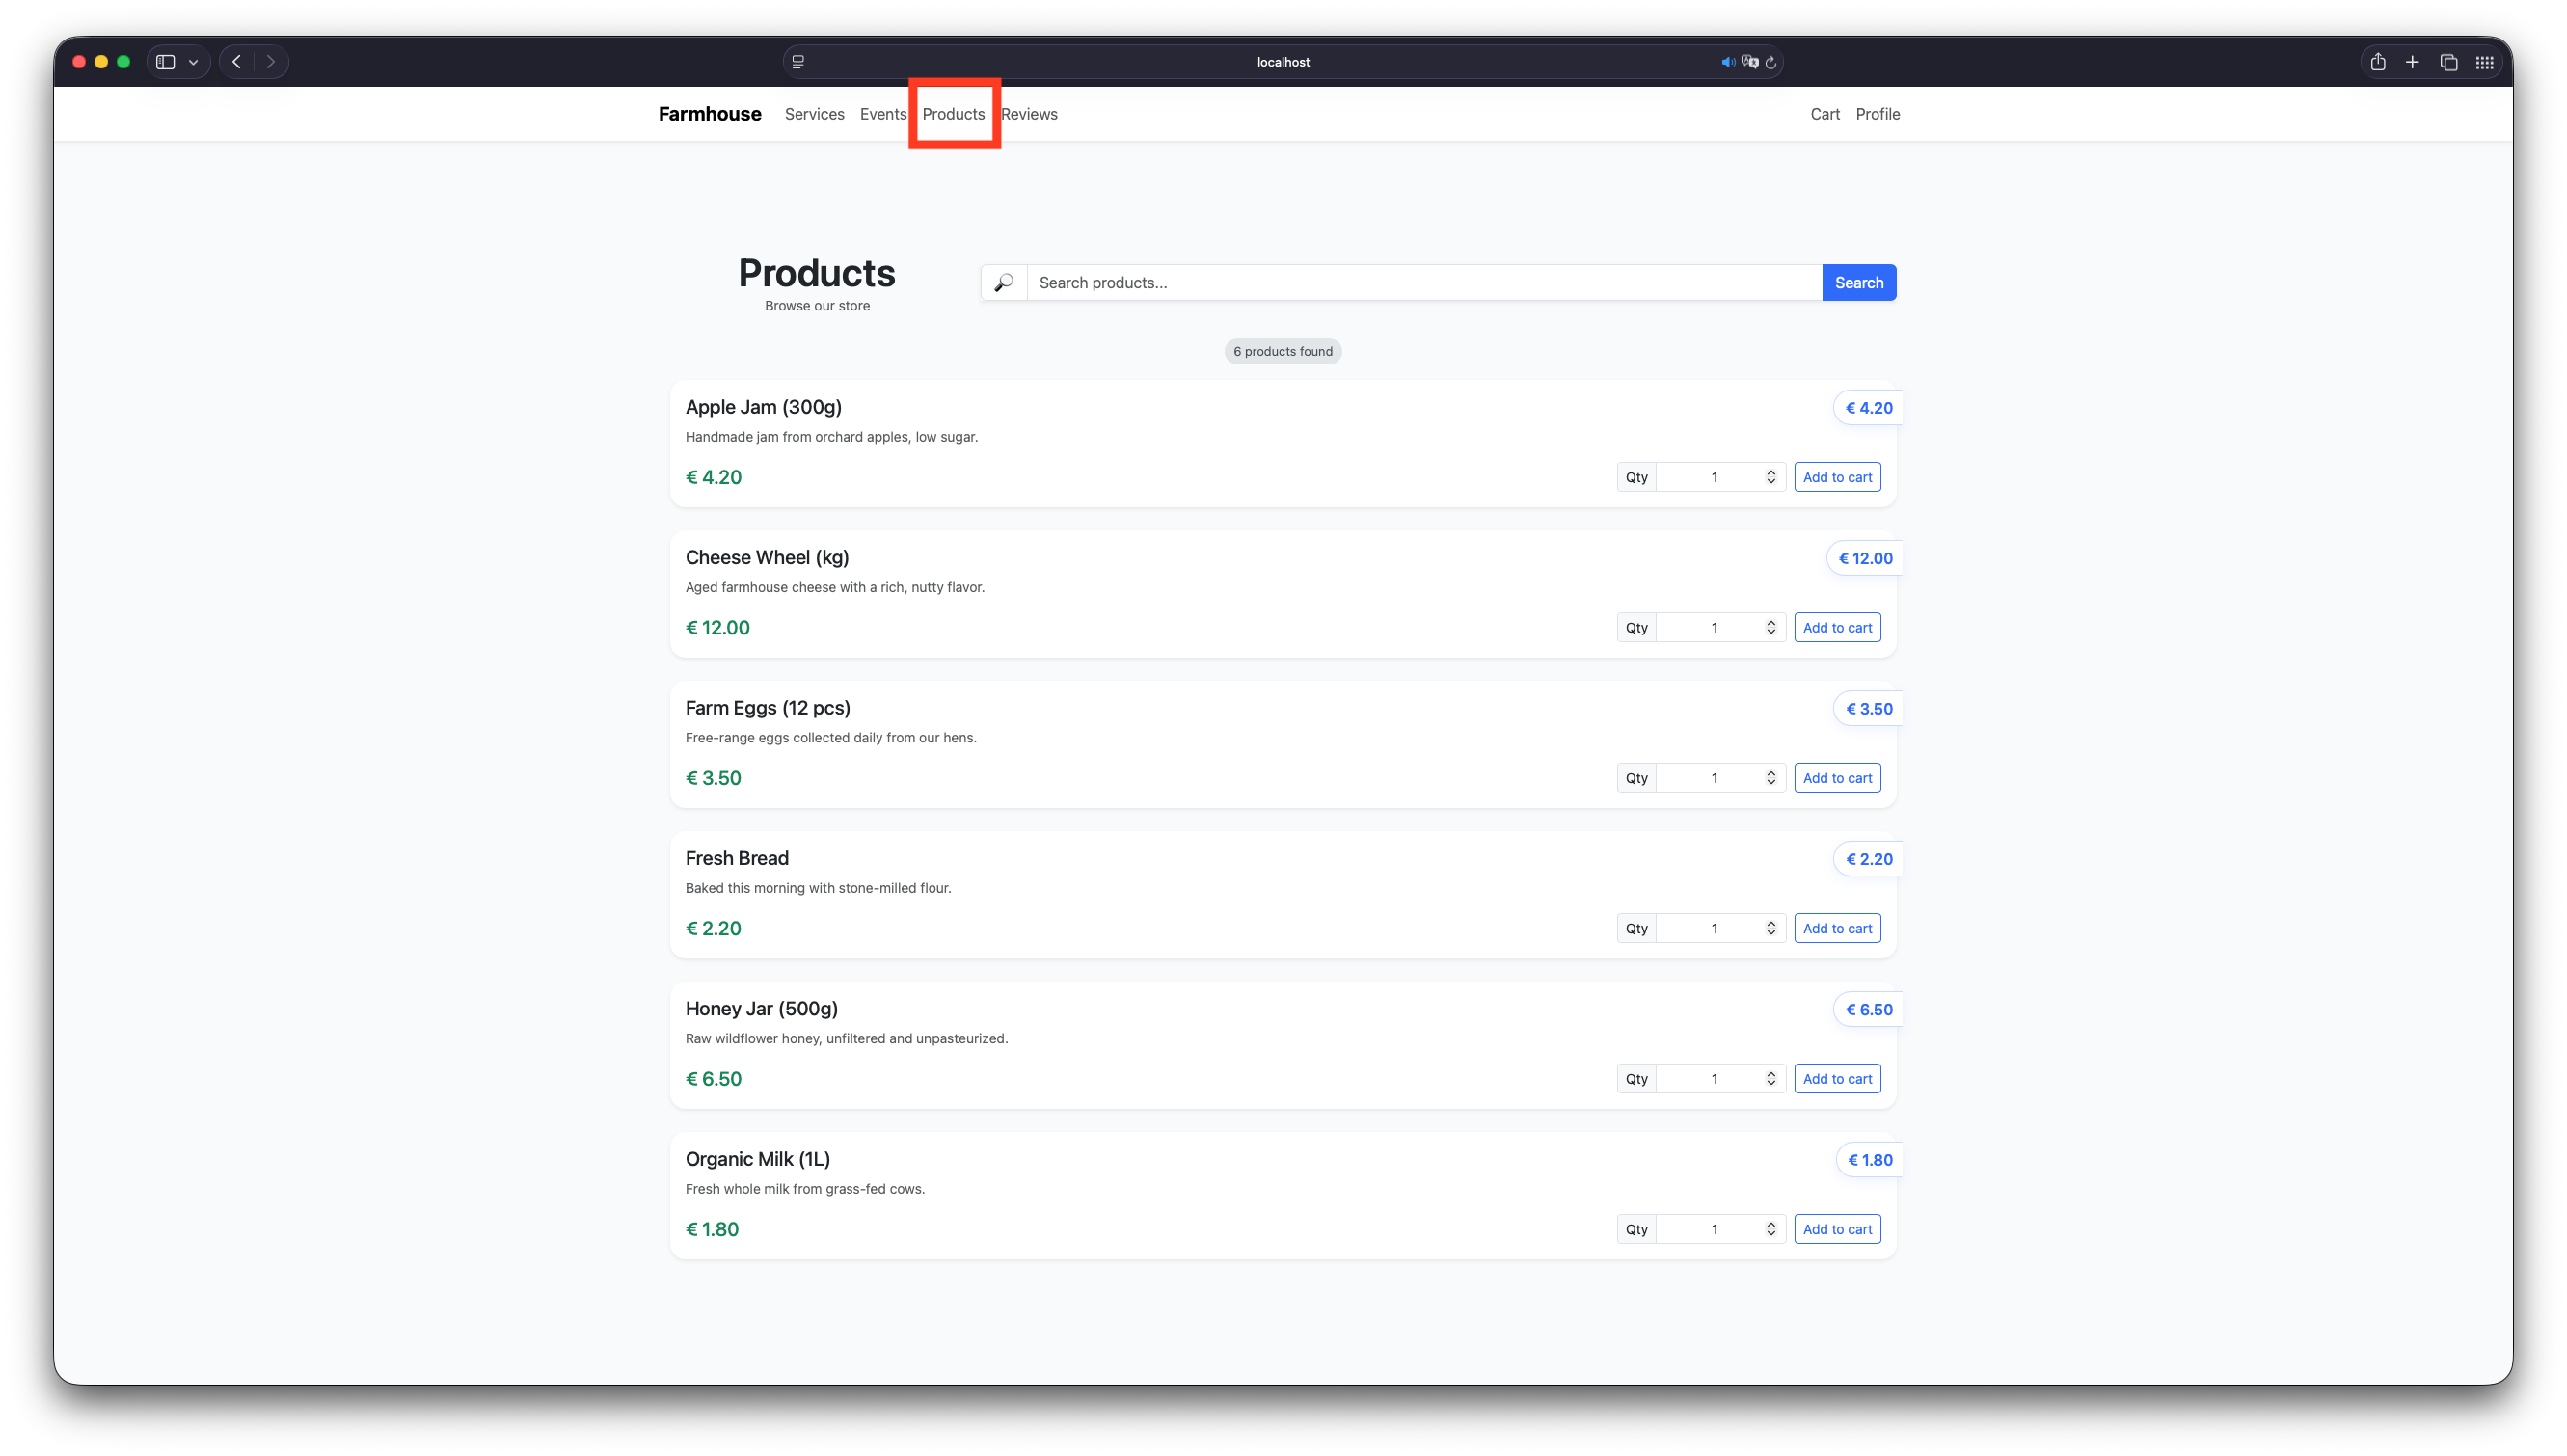
\includegraphics[width=\textwidth, trim=0 0 0 0]{./img/users/products.png}
    \vspace{-1em}
    \label{fig:products}
\end{figure}

\subsection*{Carrello}
Il \textbf{carrello} è una funzionalità applicativa che consente agli utenti di selezionare e 
gestire i prodotti da acquistare prima di confermare l'ordine. Il carrello non è rappresentato 
nel database, ma viene gestito lato applicazione: i prodotti selezionati vengono memorizzati 
temporaneamente fino al checkout, momento in cui viene creato l'ordine definitivo e 
registrato nel sistema.

\begin{figure}[H]
    \centering
    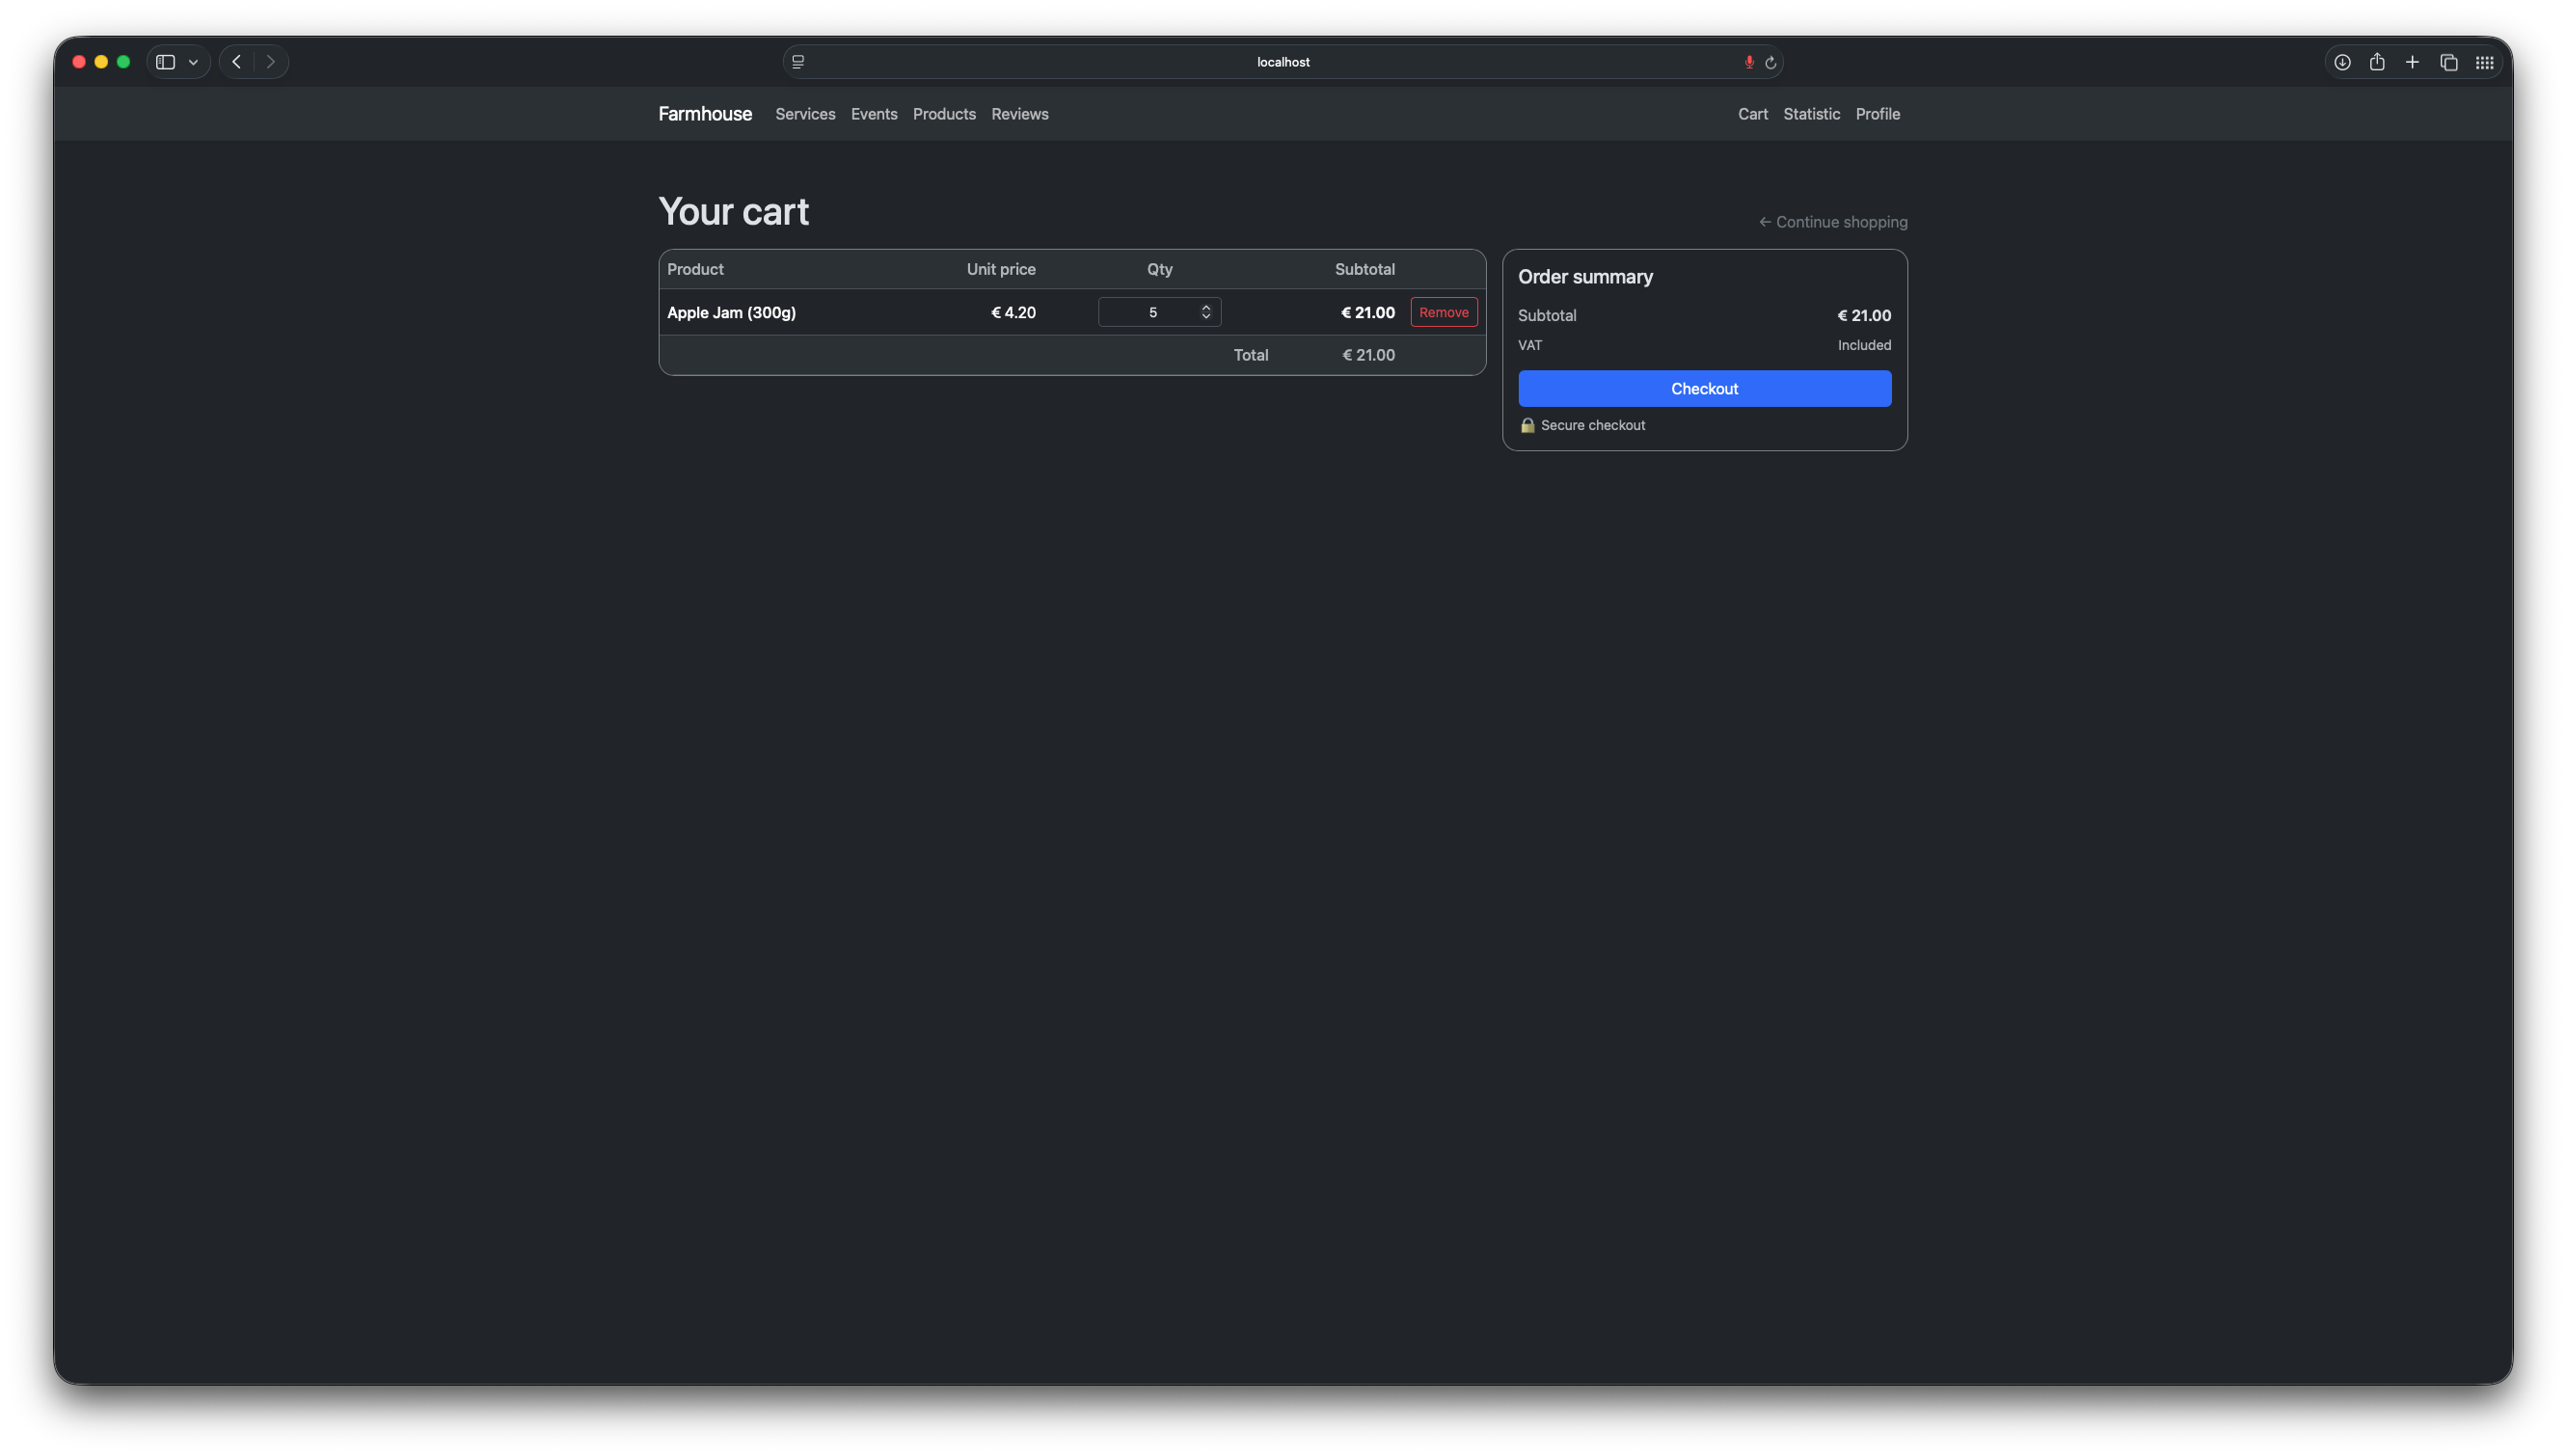
\includegraphics[width=\textwidth, trim=0 0 0 0]{./img/users/cart.png}
    \vspace{-1em}
    \label{fig:cart}
\end{figure}

\newpage
\section{Interfaccia Amministratore}
Per la gestione amministrativa, l'applicazione sfrutta la sezione \textbf{Django Admin}, 
che consente agli amministratori di accedere rapidamente a tutte le tabelle del database, 
modificare dati, tramite un'interfaccia web sicura e strutturata.

\begin{figure}[H]
    \centering
    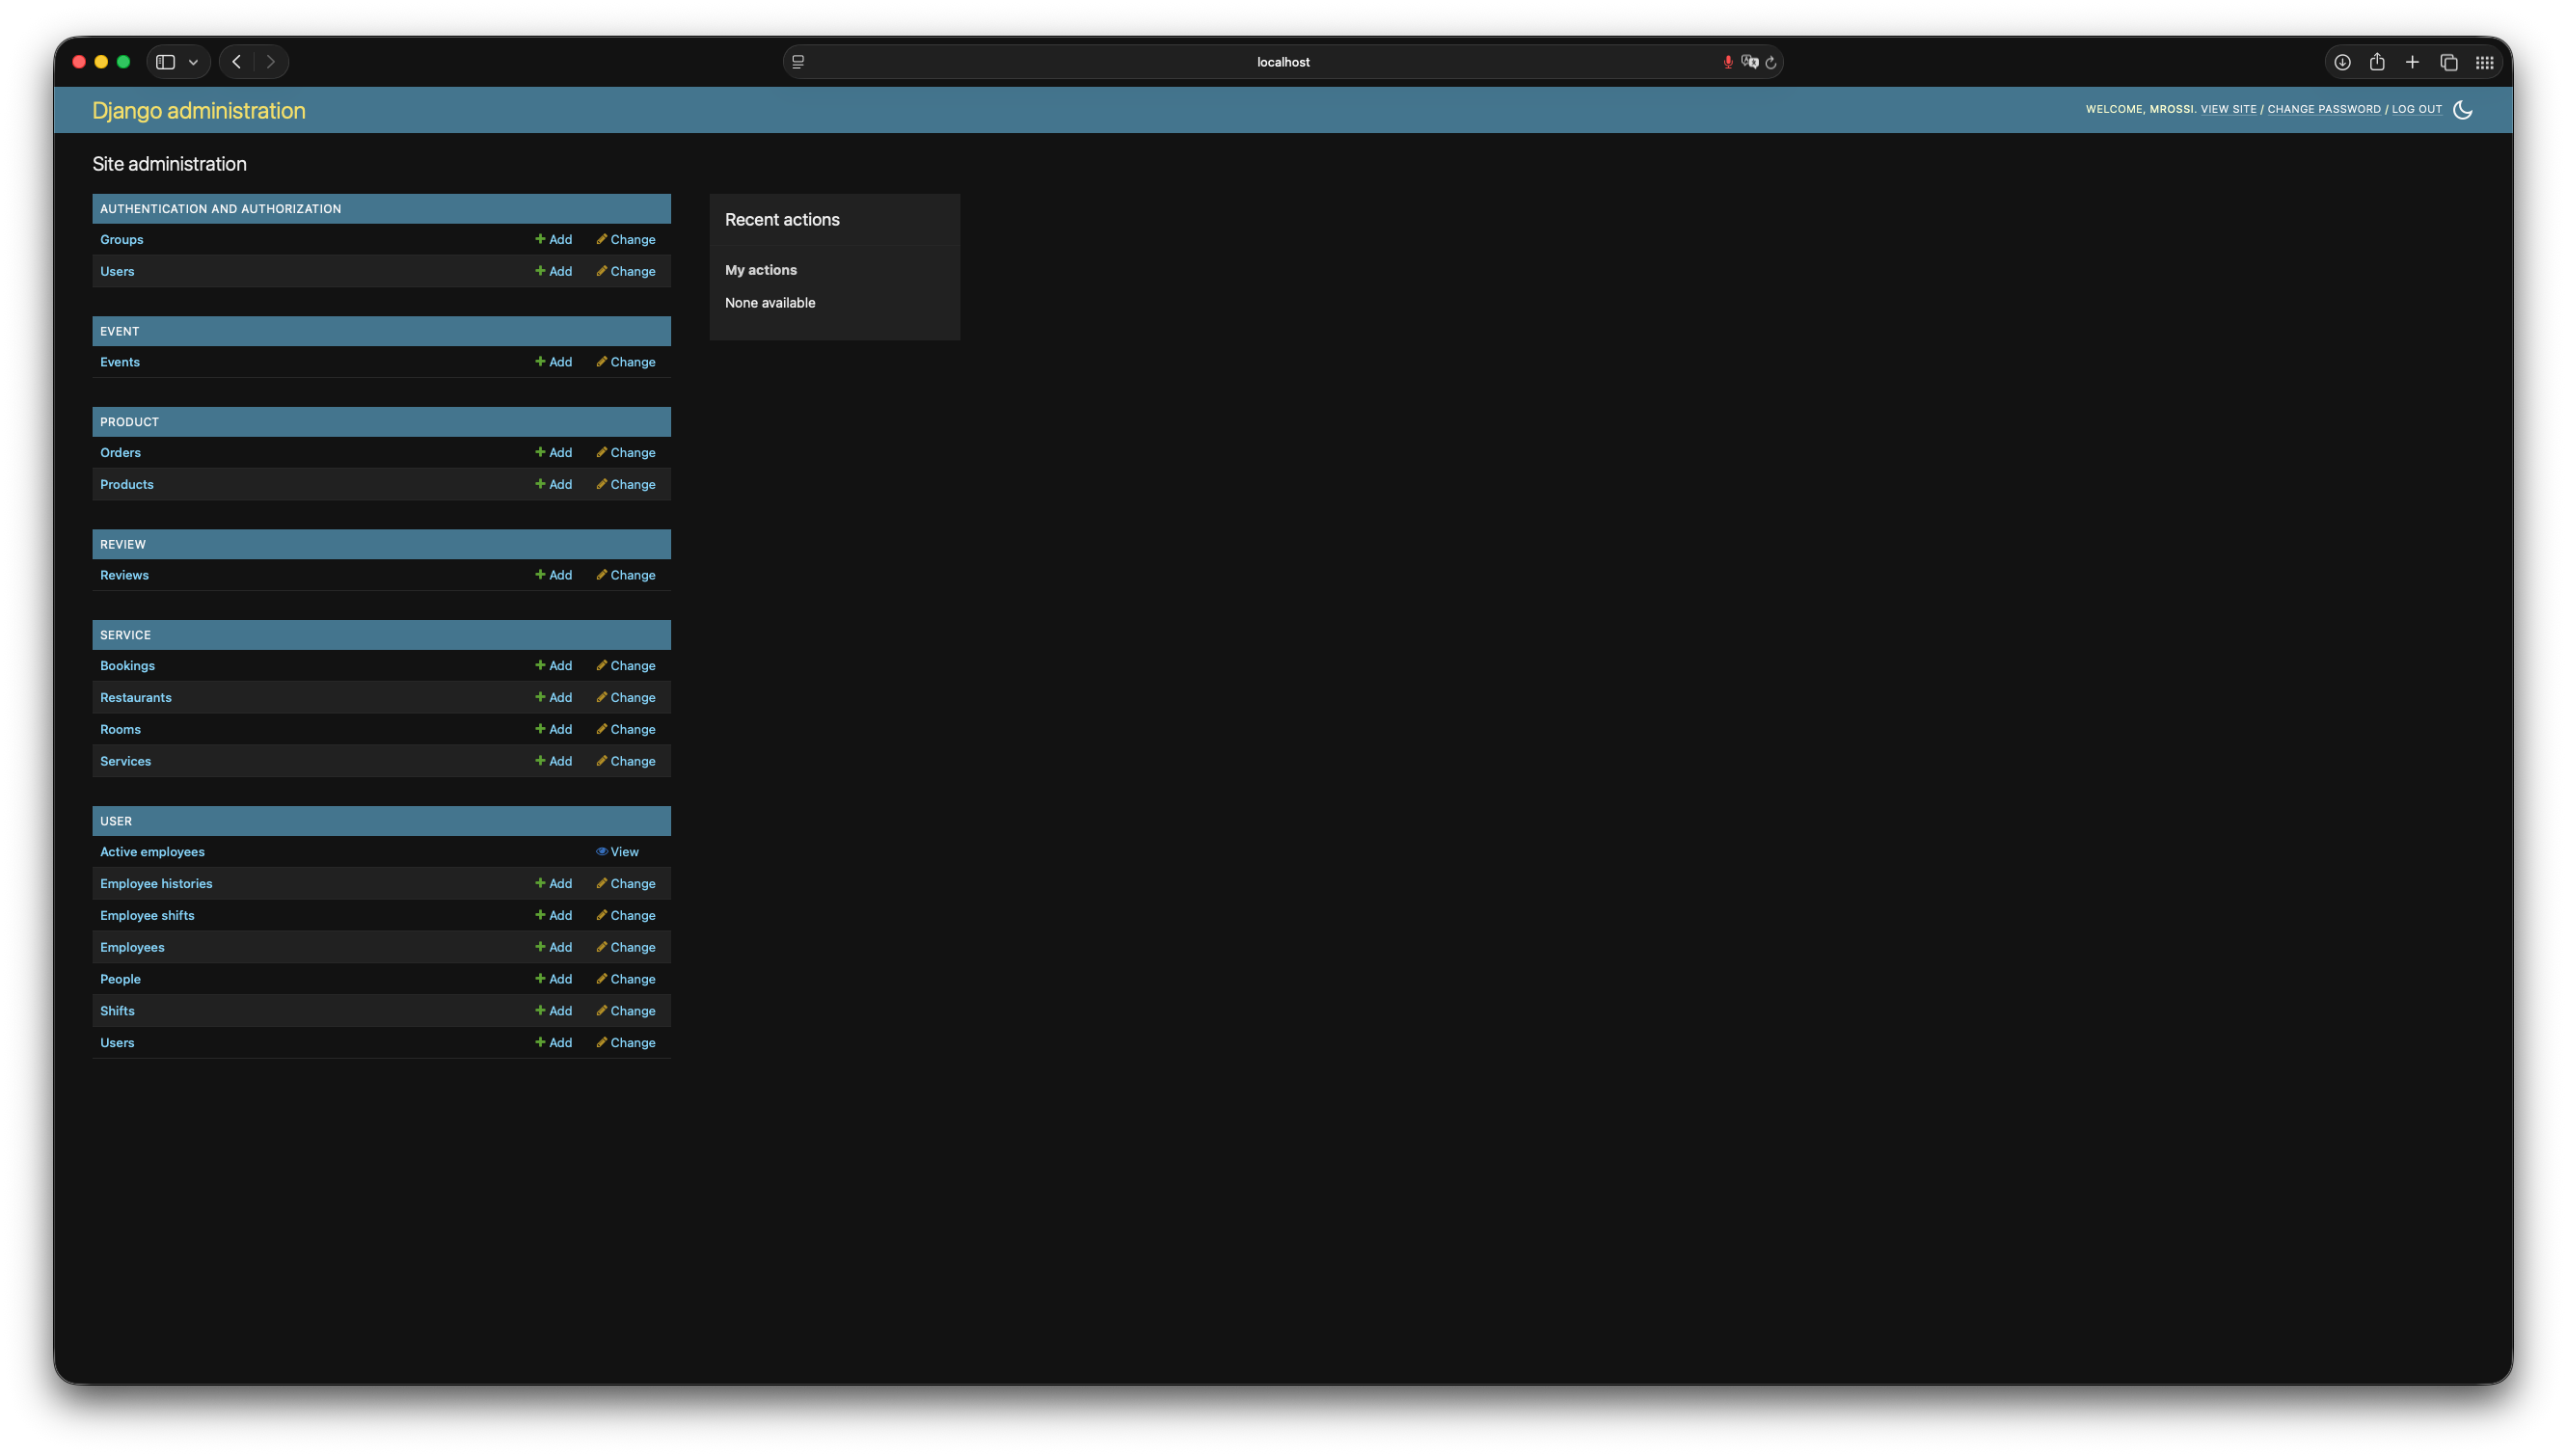
\includegraphics[width=\textwidth, trim=0 0 0 0]{./img/admin/DjangoAdmin.png}
    \vspace{-1em}
    \label{fig:django-admin}
\end{figure}

Oltre al pannello standard di Django Admin, è stata realizzata una pagina web dedicata alla 
visualizzazione delle statistiche principali del sistema, come l'andamento delle vendite, la 
partecipazione agli eventi e la presenza del personale. Questa pagina presenta tabelle 
riepilogative.

\begin{figure}[H]
    \centering
    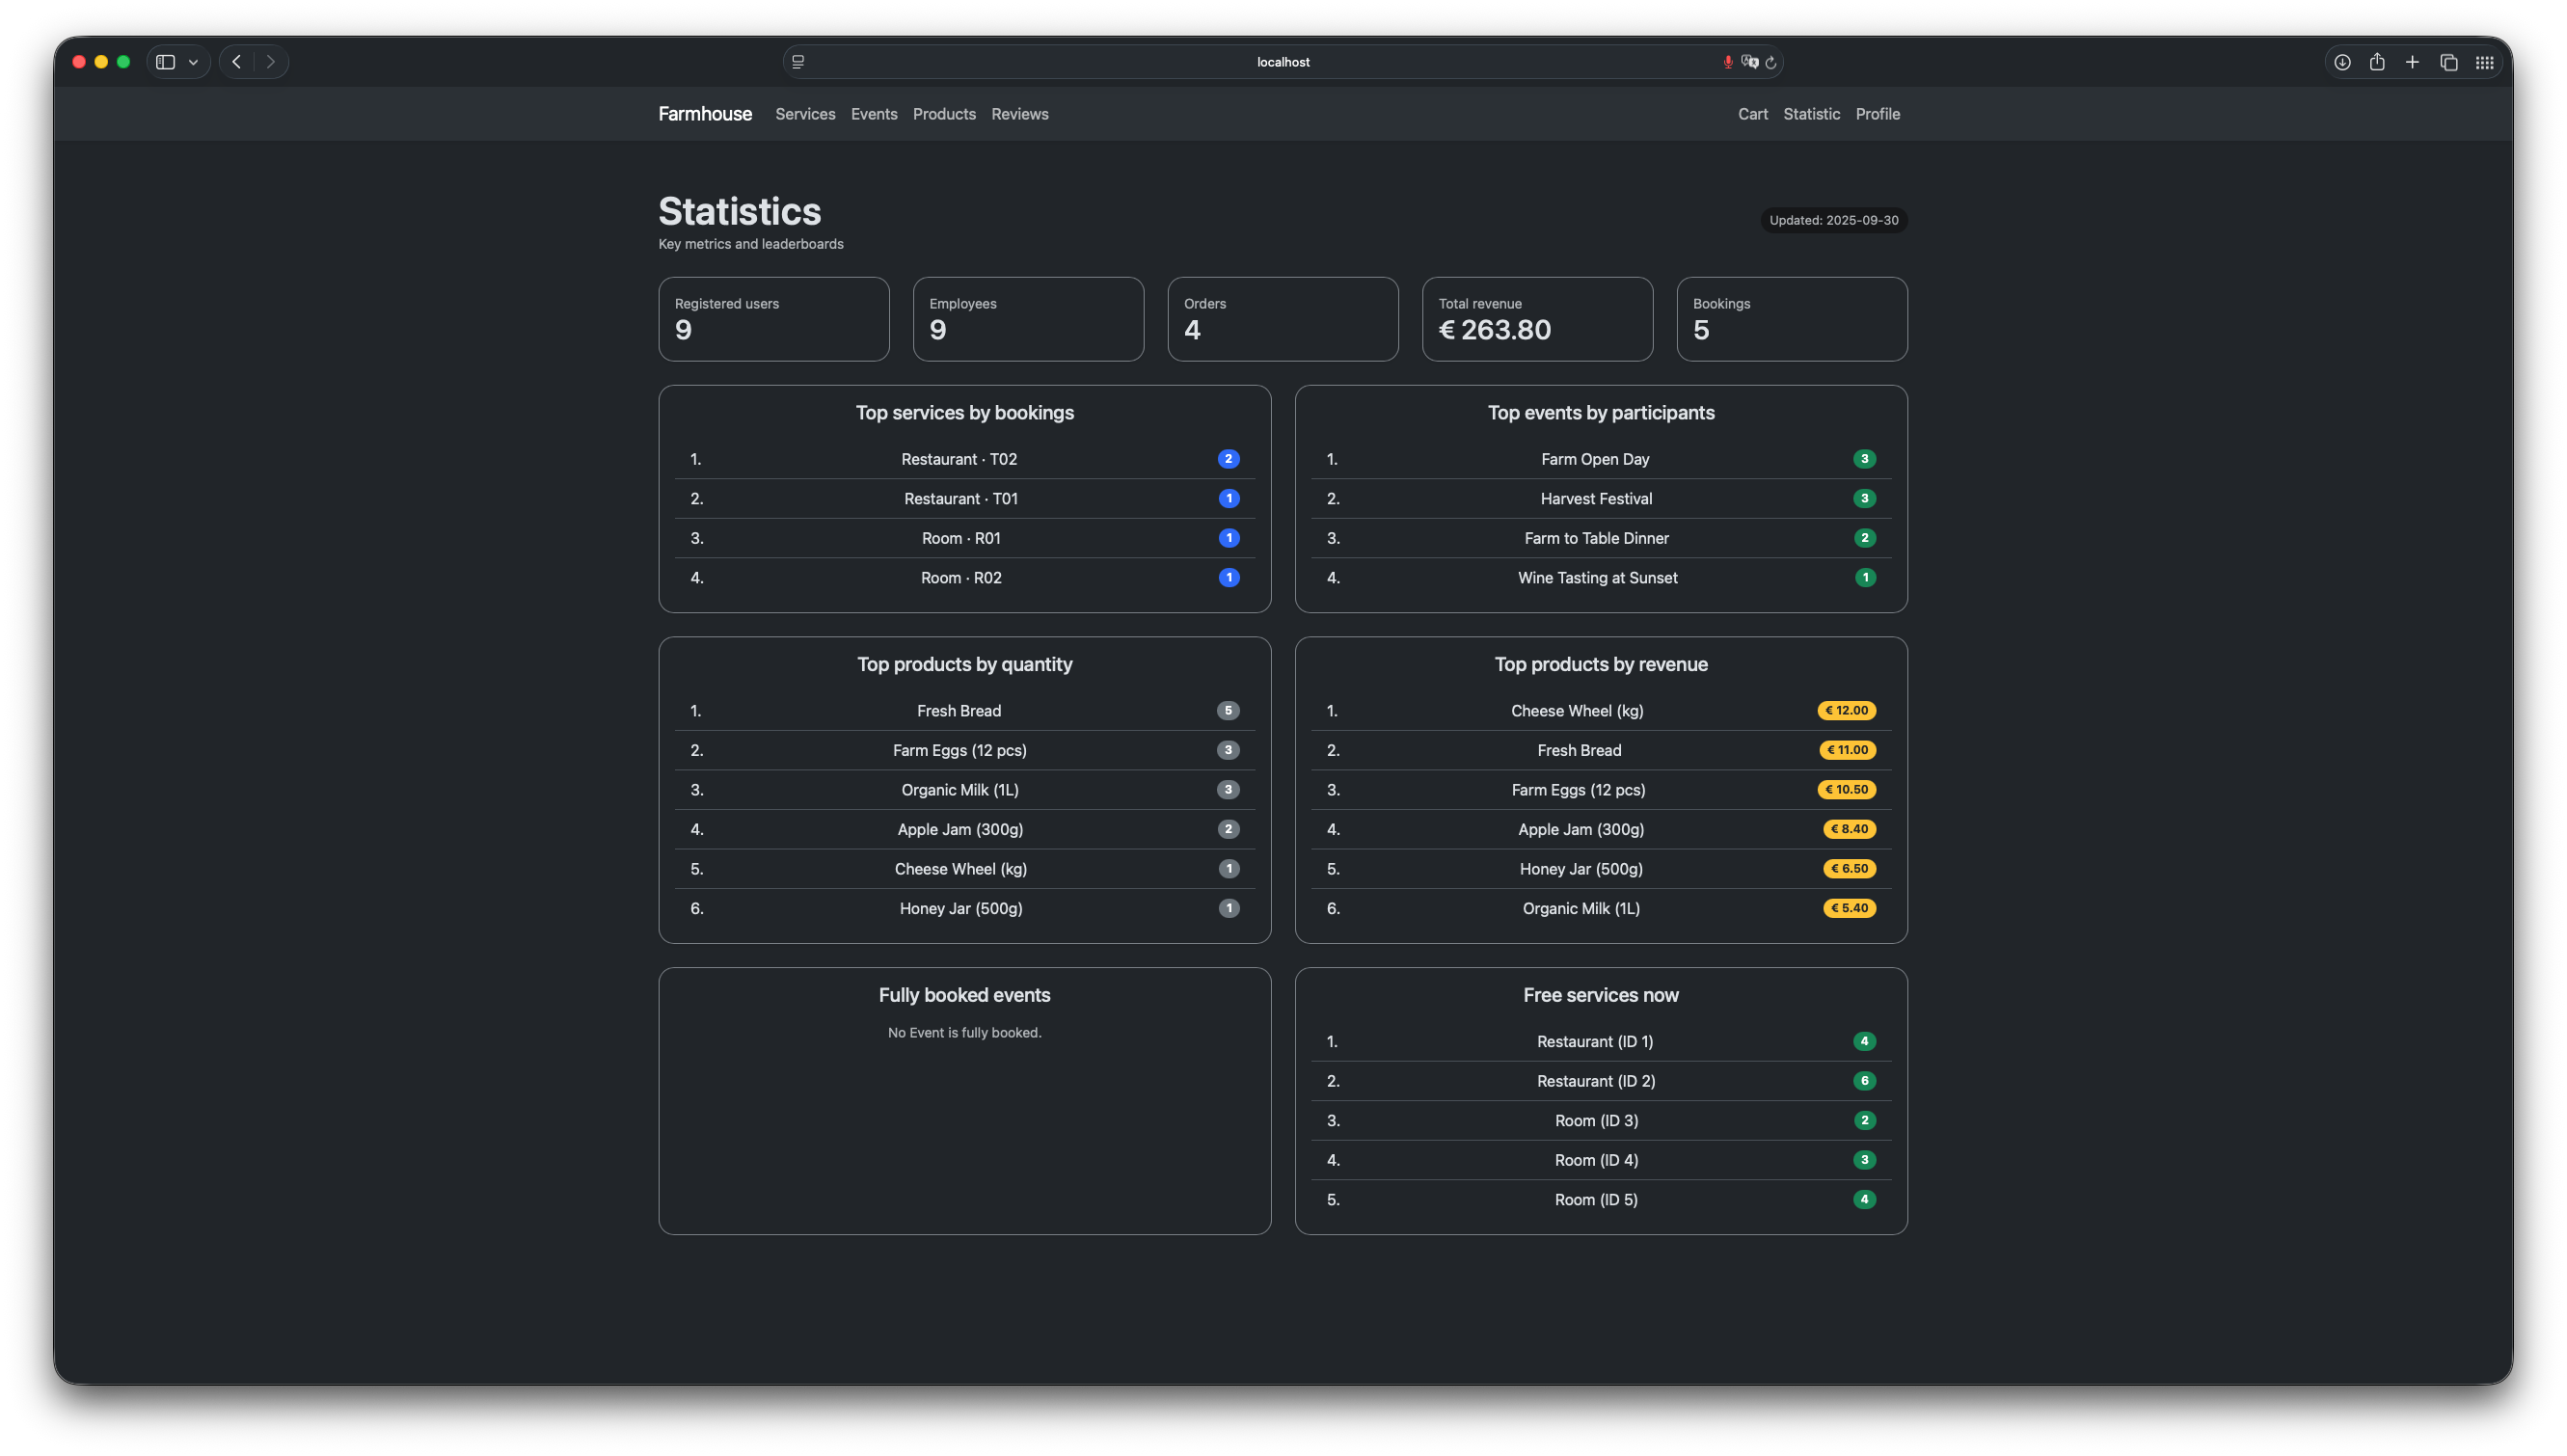
\includegraphics[width=\textwidth, trim=0 0 0 0]{./img/admin/statistic.png}
    \vspace{-1em}
    \label{fig:statistiche}
\end{figure}

\appendix
\chapter{Guida Utente}

\section{Clonazione del repository}
Clonare il progetto da GitHub e accedere alla cartella:

\begin{verbatim}
> git clone https://github.com/alessandrorebosio/D25-farmhouse.git
> cd DB25-farmhouse
\end{verbatim}

\section{Installazione delle dipendenze}

Si consiglia di utilizzare un ambiente virtuale Python per isolare le dipendenze del progetto.

\begin{verbatim}
> python3 -m venv venv
\end{verbatim}

\noindent Attivazione dell'ambiente virtuale
\begin{verbatim}
# Su Linux/macOS:
> source venv/bin/activate
# Su Windows:
> venv\Scripts\activate
\end{verbatim}

\noindent Installazione delle dipendenze dal file requirements.txt
\begin{verbatim}
> pip install -r requirements.txt
\end{verbatim}

\section{Creazione del database}

Per creare il database MySQL a partire dagli script SQL forniti, assicurarsi di avere MySQL
installato e in esecuzione.

\begin{verbatim}
> mysql -u root -p < app/sql/db.sql
> mysql -u root -p < app/sql/demo.sql
\end{verbatim}

Verrà richiesta la password dell'utente \texttt{root}. Il comando eseguirà tutte le
istruzioni SQL contenute nel file \texttt{db.sql}, creando tabelle, vincoli e dati di
esempio necessari per l'applicazione.

\section{Avvio dell'applicazione}

Per avviare l'applicazione Django, assicurarsi che l'ambiente virtuale sia attivo e che il database
sia stato creato correttamente.

\begin{verbatim}
> python manage.py migrate
> python manage.py runserver
\end{verbatim}

L'applicazione sarà accessibile all'indirizzo \url{http://localhost:8000/} tramite browser. Effettuare
il login o la registrazione per iniziare a utilizzare il sistema.

\end{document}
